%=================================================================% 
% thesis.tex																						  
%
% Updated: May 2019
%                                        
% Main file for compiler which:                                 
%	+ Defines the custom fields used in MAThesisOutputFormat.sty,
%   + Offers "final" vs "draft" formatting for speedy compiling 
%		during edits,
%   + Uses standalone package to allow the use of \input command 
%		while ignoring preambles of subfiles, 
%   + Uses BibLaTeX by default; bibtex code is in the comments, 
%   + Calls on content.tex, which contains actual content,
%   ! Uses the file thesis.bib for references,
%   ! Displays a list of tables and list of figures by default, 
%		please visit lines 279 to 281 of MAThesisOutputFormat.sty
%		to comment out the lines as necessary.
%
%=================================================================%


% Formatting commands needed for the final draft
% Note the extra space at the end, which is unfortunately necessary:      
\newcommand\myname{Patrick O'Melveny }
\newcommand\mytitle{A Volumetric Proof of the Log-Concavity of the Characteristic Polynomial of Matroids } % The graduate division requires this to be in caps.
\newcommand\mydegree{Master of Arts } % change to  Master of Science if applicable
\newcommand\myfield{Mathematics } % e.g., Mathematics
\newcommand\thismonth{December } % graduation month: May / August / December
\newcommand\thisyear{2023 } % e.g., 2014
\newcommand\myadviser{Dr.\ Dustin Ross } % Adviser
\newcommand\myadviserstitle{Assistant Professor }
\newcommand\committeememberone{Dr.\ Federico Ardila } % Committee member 1
\newcommand\committeememberonetitle{Professor } 
\newcommand\committeemembertwo{Dr.\ Matthias Beck } % Committee member 2
\newcommand\committeemembertwotitle{Professor }

\documentclass[12pt,oneside]{sfsuthesis}  


%==================================================================% 
%                                                                  %
%      WHEN THESIS IS COMPLETED, CHANGE THE NEXT LINE FROM         %    
%		                                                           % 
%		                  draft TO final,                          %
%                                                                  %
% to change format according to the Graduate Division's guidelines %
%                                                                  %
%==================================================================% 
\usepackage[draft]{MAThesisOutputFormat}
\usepackage{standalone}

%==========%
% biblatex %
%==========%
\usepackage[backend=biber,style=alphabetic]{biblatex}
\addbibresource{thesis.bib}



%=========================%
% CUSTOM COMMANDS GO HERE %
%=========================%
%====================%
% Packages 
%====================%
%\usepackage{accents}  % Better accents. I'm not using this
\usepackage{enumitem} % Better labels
%\usepackage[explicit]{titlesec}
\usepackage[normalem]{ulem}     % Thing
\usepackage{stackrel} % Stack text nicely
\usepackage{xcolor}   % Nicer Colors

%====================%
% Re-Define 
%====================%
% Sort out the true phi
\def \badphi {\phi}
\def \phi {\varphi}

%====================%
% New Commands 
%====================%
%% Nice Letters
% Blackboard Bold
\newcommand{\R}{\mathbb{R}}
\newcommand{\Z}{\mathbb{Z}}
\newcommand{\bbS}{\mathbb{S}}
% Fancy Math Cal Letters
\newcommand{\I}{\mathcal{I}}
\newcommand{\J}{\mathcal{J}}
\newcommand{\cL}{\mathcal{L}}
\newcommand{\cF}{\mathcal{F}}
% The hipster letters
\newcommand{\sM}{\mathsf{M}}
\newcommand{\bSigma}{\boldsymbol{\Sigma}}
\newcommand{\ow}{\overline{w}}
\newcommand{\oP}{\overline{P}}
\newcommand{\oQ}{\overline{Q}}
\newcommand{\ochi}{\overline{\chi}}
%% Math Operators
\newcommand{\Cub}{\operatorname{Cub}}
\newcommand{\oCub}{\overline{\Cub}}
\newcommand{\Vol}{\operatorname{Vol}}
\newcommand{\oVol}{\overline{\Vol}}
\newcommand{\MVol}{\operatorname{MVol}}
%% Math Symbols
\newcommand{\cl}{\mathrm{cl}}
\newcommand{\rk}{\mathrm{rk}}
\newcommand{\Inn}{\mathrm{Inn}}
\newcommand{\cone}{\mathrm{cone}}

%====================%
% Theorem Environs
%====================%
\newtheorem{dummy}{}[section]
\theoremstyle{definition}
\newtheorem*{Result}{Main Result}

%====================%
% Draft Helpers
%====================%
% \todo : Make a box with todo comments
\newcommand{\todo}[1]{\par \noindent
    \framebox{\begin{minipage}[c]{0.95 \textwidth}
            \textcolor{red}{TO DO:}
            #1 \end{minipage}}\par}

%================================%
%             Thesis             %
%================================%
\begin{document}

%==============%
%     Title    %
%==============%
\thesistitle%

%====================%
%       To-do        %
%====================%
%\listoftodos%

%==============%
%   Chapeters  %
%==============%
\documentclass[12pt,oneside]{../../sfsuthesis}  

\RequirePackage{standalone}
\usepackage[draft]{../../MAThesisOutputFormat}
%====================%
% Packages 
%====================%
%\usepackage{accents}  % Better accents. I'm not using this
\usepackage{enumitem} % Better labels
%\usepackage[explicit]{titlesec}
\usepackage[normalem]{ulem}     % Thing
\usepackage{stackrel} % Stack text nicely
\usepackage{xcolor}   % Nicer Colors

%====================%
% Re-Define 
%====================%
% Sort out the true phi
\def \badphi {\phi}
\def \phi {\varphi}

%====================%
% New Commands 
%====================%
%% Nice Letters
% Blackboard Bold
\newcommand{\R}{\mathbb{R}}
\newcommand{\Z}{\mathbb{Z}}
\newcommand{\bbS}{\mathbb{S}}
% Fancy Math Cal Letters
\newcommand{\I}{\mathcal{I}}
\newcommand{\J}{\mathcal{J}}
\newcommand{\cL}{\mathcal{L}}
\newcommand{\cF}{\mathcal{F}}
% The hipster letters
\newcommand{\sM}{\mathsf{M}}
\newcommand{\bSigma}{\boldsymbol{\Sigma}}
\newcommand{\ow}{\overline{w}}
\newcommand{\oP}{\overline{P}}
\newcommand{\oQ}{\overline{Q}}
\newcommand{\ochi}{\overline{\chi}}
%% Math Operators
\newcommand{\Cub}{\operatorname{Cub}}
\newcommand{\oCub}{\overline{\Cub}}
\newcommand{\Vol}{\operatorname{Vol}}
\newcommand{\oVol}{\overline{\Vol}}
\newcommand{\MVol}{\operatorname{MVol}}
%% Math Symbols
\newcommand{\cl}{\mathrm{cl}}
\newcommand{\rk}{\mathrm{rk}}
\newcommand{\Inn}{\mathrm{Inn}}
\newcommand{\cone}{\mathrm{cone}}

%====================%
% Theorem Environs
%====================%
\newtheorem{dummy}{}[section]
\theoremstyle{definition}
\newtheorem*{Result}{Main Result}

%====================%
% Draft Helpers
%====================%
% \todo : Make a box with todo comments
\newcommand{\todo}[1]{\par \noindent
    \framebox{\begin{minipage}[c]{0.95 \textwidth}
            \textcolor{red}{TO DO:}
            #1 \end{minipage}}\par}
\usepackage[backend=biber,style=numeric]{biblatex}
\addbibresource{../../thesis.bib}

\begin{document}

\chapter{Introduction}

\todo{Add Citations in Introduction}

This thesis will require us to take a tour of mathematics that have been developing for close to a century.
The main result synthesizes modern work, from about ten years right up to last year, about a conjecture, posed in seventies, on a mathematical object first formalized in 1935.
This threads through work of our friends and mentors, Fields Medal winners, and a host of well-known mathematicians from across the last hundred years.
While we think the results alone are quite interesting on their own, much of what has made this project so interesting to us is its broad connections to these various places.
We hope, through the more leisurely pace we are allowed to take in a thesis, to show off this side of the math as well.

\section{What Are We Doing?}

The key players in this work are \textbf{matroids}, a combinatorial object devised to generalize the notion of ``independence''.
Matroids are interesting for a multitude of reasons, but of note to us is that, although they are combinatorial objects, they can be alternatively studied as geometric objects, known as \textbf{Bergmann fans}, and algebraic objects, polynomials rings called \textbf{Chow rings}.
In the early 1970's, a conjecture about the \textbf{characteristic polynomial} of matroids was posed.
The \textbf{Heron-Rota-Welsh conjecture} was, in essence a combinatorial question, and would remain unresolved for almost 50 years.
It was through viewing the problem from the algebro-geometric side of things that Adiprasito, Huh, and Katz were finally able to prove the conjecture true in 2017.
They did this by importing complex machinery from algebraic geometry, known as \emph{Hodge theory}, into the combinatorial world of matroids.
It is an impressive work that, in part, won author June Huh a Fields medal.

In this thesis we wish to offer an alternative proof of the Heron-Rota-Welsh conjecture.
To do this, we too will tackle the problem from a geometric perspective.
In 2021, Nathanson and Ross developed a correspondence between the volume of objects generated from the Bergmann fans of matroids, called \textbf{normal complexes}, and the evaluation of degree maps on the Chow Ring.
This opened the avenue of using the geometric picture of matroids to show characteristics of its algebraic representation.
Using the recent work of Nowak, O\todo{It feels weird to use my name in the 3rd person?}, and Ross, we show this correspondence and certain volumetric properties of normal complexes is sufficient to prove the Heron-Rota-Welsh conjecture.

\section{Why Are We Doing This?}

Where some would ask why, we much prefer to ask ``why not?''.
More seriously, while \textit{a} proof of the Heron-Rolta-Welsh conjecture is not new, having a new viewpoint on something is valuable even just in comparing it to the original.

This is an exciting starting application of the theory of normal complexes.
Compared to combinatorial Hodge theory, normal complexes have a much lower barrier of entry.
That they can prove the same, famously difficult, problem is surprising at least.
We hope to see some of these techniques and tools expanded and applied elsewhere.

\section{Who Is This For?}

By this point we've already introduced quite a few words we don't expect every reader to know offhand.
Our primary goal is that anyone with a few graduate level courses in mathematics under their belt could read this thesis from start to finish and come out with a comprehensive picture of both the setting and the conclusion.
To that end we will be providing context for every word in bold appearing above, linking each of them to the overall picture.

However, we also have some secondary goals in terms of readership.
First, we want this to be of at least some interest to someone already knowledgeable in the field.
While we are confident that any math of real substance in this thesis will be developed elsewhere, if it's going to appear here it might as well at least be useful to a practitioner.
Second, and in somewhat of a contradiction, we want this work to be inviting to a curious non-mathematican.
We believe there is a good opportunity here to allow a layperson to follow along with math they may not be otherwise usually exposed too.

In the true spirit of compromise then, we expect no one to be totally happy with the pacing.
In general, the intention is the complexity of the material will start somewhat low and increase as we go on.
But, there will be technical points interjected in otherwise easy material, and we will attempt to include high level overviews even in sections that really do require a solid mathematical background.
We say this largely to give the reader permission to skip the bits that simply don't interest them.
%However you engage with this thesis, we hope a reader gets something out of it.
%Even better if they were to somewhat enjoy the process.

\end{document}

\documentclass[12pt,oneside]{../../sfsuthesis}  

\RequirePackage{standalone}
\usepackage[draft]{../../MAThesisOutputFormat}
%====================%
% Packages 
%====================%
%\usepackage{accents}  % Better accents. I'm not using this
\usepackage{enumitem} % Better labels
%\usepackage[explicit]{titlesec}
\usepackage[normalem]{ulem}     % Thing
\usepackage{stackrel} % Stack text nicely
\usepackage{xcolor}   % Nicer Colors

%====================%
% Re-Define 
%====================%
% Sort out the true phi
\def \badphi {\phi}
\def \phi {\varphi}

%====================%
% New Commands 
%====================%
%% Nice Letters
% Blackboard Bold
\newcommand{\R}{\mathbb{R}}
\newcommand{\Z}{\mathbb{Z}}
\newcommand{\bbS}{\mathbb{S}}
% Fancy Math Cal Letters
\newcommand{\I}{\mathcal{I}}
\newcommand{\J}{\mathcal{J}}
\newcommand{\cL}{\mathcal{L}}
\newcommand{\cF}{\mathcal{F}}
% The hipster letters
\newcommand{\sM}{\mathsf{M}}
\newcommand{\bSigma}{\boldsymbol{\Sigma}}
\newcommand{\ow}{\overline{w}}
\newcommand{\oP}{\overline{P}}
\newcommand{\oQ}{\overline{Q}}
\newcommand{\ochi}{\overline{\chi}}
%% Math Operators
\newcommand{\Cub}{\operatorname{Cub}}
\newcommand{\oCub}{\overline{\Cub}}
\newcommand{\Vol}{\operatorname{Vol}}
\newcommand{\oVol}{\overline{\Vol}}
\newcommand{\MVol}{\operatorname{MVol}}
%% Math Symbols
\newcommand{\cl}{\mathrm{cl}}
\newcommand{\rk}{\mathrm{rk}}
\newcommand{\Inn}{\mathrm{Inn}}
\newcommand{\cone}{\mathrm{cone}}

%====================%
% Theorem Environs
%====================%
\newtheorem{dummy}{}[section]
\theoremstyle{definition}
\newtheorem*{Result}{Main Result}

%====================%
% Draft Helpers
%====================%
% \todo : Make a box with todo comments
\newcommand{\todo}[1]{\par \noindent
    \framebox{\begin{minipage}[c]{0.95 \textwidth}
            \textcolor{red}{TO DO:}
            #1 \end{minipage}}\par}
\usepackage[backend=biber,style=numeric]{biblatex}
\addbibresource{../../thesis.bib}

\begin{document}


\chapter{Matriods}

Much of our concern is around matroids, so best we get a clear idea of what one is.

\section{What is a Matroid?}


and things!
\end{document}

\documentclass[12pt,oneside]{../../sfsuthesis} 
 
\RequirePackage{standalone}
\usepackage[draft]{../../MAThesisOutputFormat}
%====================%
% Packages 
%====================%
%\usepackage{accents}  % Better accents. I'm not using this
\usepackage{enumitem} % Better labels
%\usepackage[explicit]{titlesec}
\usepackage[normalem]{ulem}     % Thing
\usepackage{stackrel} % Stack text nicely
\usepackage{xcolor}   % Nicer Colors

%====================%
% Re-Define 
%====================%
% Sort out the true phi
\def \badphi {\phi}
\def \phi {\varphi}

%====================%
% New Commands 
%====================%
%% Nice Letters
% Blackboard Bold
\newcommand{\R}{\mathbb{R}}
\newcommand{\Z}{\mathbb{Z}}
\newcommand{\bbS}{\mathbb{S}}
% Fancy Math Cal Letters
\newcommand{\I}{\mathcal{I}}
\newcommand{\J}{\mathcal{J}}
\newcommand{\cL}{\mathcal{L}}
\newcommand{\cF}{\mathcal{F}}
% The hipster letters
\newcommand{\sM}{\mathsf{M}}
\newcommand{\bSigma}{\boldsymbol{\Sigma}}
\newcommand{\ow}{\overline{w}}
\newcommand{\oP}{\overline{P}}
\newcommand{\oQ}{\overline{Q}}
\newcommand{\ochi}{\overline{\chi}}
%% Math Operators
\newcommand{\Cub}{\operatorname{Cub}}
\newcommand{\oCub}{\overline{\Cub}}
\newcommand{\Vol}{\operatorname{Vol}}
\newcommand{\oVol}{\overline{\Vol}}
\newcommand{\MVol}{\operatorname{MVol}}
%% Math Symbols
\newcommand{\cl}{\mathrm{cl}}
\newcommand{\rk}{\mathrm{rk}}
\newcommand{\Inn}{\mathrm{Inn}}
\newcommand{\cone}{\mathrm{cone}}

%====================%
% Theorem Environs
%====================%
\newtheorem{dummy}{}[section]
\theoremstyle{definition}
\newtheorem*{Result}{Main Result}

%====================%
% Draft Helpers
%====================%
% \todo : Make a box with todo comments
\newcommand{\todo}[1]{\par \noindent
    \framebox{\begin{minipage}[c]{0.95 \textwidth}
            \textcolor{red}{TO DO:}
            #1 \end{minipage}}\par}
\usepackage[backend=biber,style=alphabetic]{biblatex}
\addbibresource{../../thesis.bib}

\begin{document}

\chapter{Chow Rings}

It is time now to delve into the world of algebra, developing the notion of a Chow ring of a matroid.
The primary goal of this section will be to establish the link between the Chow ring and the characteristic polynomial.
This will form the first segment of our bridge from combinatorics to geometry.

This section will take some algebraic knowledge for granted; we're not going to define a ring, for example.
The main takeaway will be in the last section and should be enough to move on to the next chapter.
However, even for those with some basic algebra we don't expect Chow rings to be a familiar object, so our first order of business is to define them.

\section{What is a Chow Ring?}

Broadly, Chow rings are a tool from algebraic geometry for studying the intersections of algebraic varieties.
Chow groups of an algebraic variety are equivalence classes of algebraic cycles of its subvarieties, graded by their codimension.
They were named after Wei-Liang Chow, who formalized these cycles in \cite{chowEquivalenceClassesCycles1956}.
Under certain conditions, a product structure can be induced on these groups to give a ring, which encodes additional information about the intersections of the subvarieties.

For those who don't already have some idea of what a Chow ring is, the above probably invites more questions than it clarifies.
Happily, as hinted by the fact that the title of this chapter is not ``A Brief Introduction to Algebraic Geometry and Intersection Theory'', we will not have to tackle the full theory to get a result here.
While there are algebraic varieties hiding in the wings, we will see that the combinatorial data of a matroid allow us to define its corresponding Chow ring quite directly.

\subsection{The Chow Ring of a Matroid}

For our purposes, we will define the Chow ring to be this ``short-cut'' construction.
That this construction corresponds to the idea of the Chow ring presented above comes from the work started by De Cocini and Procesi \cite{deconciniWonderfulModelsSubspace1995} and generalized to the form we will use by Feichtner and Yuzvinsky \cite{feichtnerChowRingsToric2004}.
\begin{definition}[The Chow Ring of a Matroid]\label{def:chowRing}
    Let \( \cM = (E, \cL)\) be a matroid.
    Associate a polynomial ring with \( \cM \) given by
    \[
        P_\cM = \R[x_F \; | \; F \in \cL^\ast],
    \]
    and let
    \begin{align*}
        I_\cM & = \left\langle x_{F_1}x_{F_2} \; \middle| \; F_1 \not\subseteq F_2\, \text{and}\, F_2 \not\subseteq F_1 \right\rangle, \\
        J_\cM & = \left\langle \sum_{e_1 \in F} x_{F} - \sum_{e_2 \in F} x_{F} \; \middle| \; e_1, e_2 \in E \right\rangle
    \end{align*}
    be ideals of \(P_\cM\).

    The \emph{Chow ring of \( \cM \)} is given by the quotient
    \[
        A^{\bullet}(\cM) = \frac{P_{\cM}}{I_{\cM} + J_{\cM}}.
    \]
\end{definition}

By way of some intuition building, the idea here is to create a polynomial ring with variables corresponding to the proper flats of our matroid, then encode the combinatorial relations of the matroid using a quotient.
We could think of the ideal \( I_{\cM} \) as telling us that any monomial involving flats that don't form a flag are removed.
The ideal \( J_{\cM} \) has a less obvious intuition, but the linear forms that generate it give us useful relations that we will use later.
As always, working a small example will help.

\subsubsection{A Small Chow Ring Example}
Recall our ongoing example matroid \( \cM \), whose ground set is \( E = \{ a,b,c,d \} \) and with proper flats
\[
    \cL^\ast = \{ a, b, c, d, abd, ac, bc, cd \}.
\]

Then we have the polynomial ring
\[
    P_{\cM} = \R[x_{a}, x_{b}, x_{c}, x_{d}, x_{abd}, x_{ac}, x_{bc}, x_{cd}];
\]
i.e.\ a real polynomial ring in 8 variables.
Elements of the ideal \( I_{\cM} \) will be any multiple of a monomial containing variables corresponding to non-comparable flats, such as
\[
    x_a x_d \in I_{\cM} \quad \text{and} \quad x_c x_{abd} \in I_{\cM}.
\]
The ideal \( J_{\cM} \) in turn is generated from differences of sums of all variables that contain a particular ground element. For example,
\begin{align*}
    \sum_{a \in F}x_F - \sum_{c \in F}x_F & = x_a + x_{abd} + x_{ac} - x_c - x_{ac} - x_{cd} \\
                                          & = x_a + x_{abd} - x_c - x_{cd} \in J_{\cM}.
\end{align*}

Now, elements in our Chow ring \( A^\bullet(\cM) \) are equivalence classes, as expected for a quotient ring.
We see that \( J_\cM \) gives us relations like
\[
    [x_a + x_{abd}] = [x_c + x_{cd}],
\]
or, equivalently,
\[
    [x_a] = [x_c + x_{cd} - x_{abd}].
\]

In continuing to strive for succinct notation, we will drop the square brackets on elements of the Chow ring going forward.

\section{The Degree Map}

Now that we have an idea of what the Chow ring is, we can introduce the next key idea, the degree map.
However, to get to the degree map we will need the property that Chow rings are graded.

\subsection{This Will Be Graded}
Our goal here to show that the Chow ring is a graded ring.
Those that feel that this property is obvious can skip to the next section; for everyone else we'll provide a quick summary.
\begin{definition}[Graded Ring]
    A ring \( R \) is \emph{graded} if the underlying additive group of \( R \) can be decomposed into a direct sum
    \[
        R = \bigoplus_{i=0}^\infty R_i
    \]
    where each \( R_i \) is an abelian group such that \( R_i R_j \subseteq R_{i+j} \) for all \( i, j \in \Z_{\geq 0}\).
    Elements of \( R_i \) are called \emph{homogeneous of degree \( i \)}.
\end{definition}
From this definition we can see that any polynomial ring, \( P \) is a graded ring
\[
    P =  \bigoplus_{i=0}^\infty P_i
\]
where each \( P_i \) is, naturally, all homogeneous polynomials of degree \( i \).

Additionally, we can define a specific kind of ideal for graded rings, homogeneous ideals.
\begin{definition}[Homogeneous Ideals]
    Let \( R \) be a graded ring. An ideal \( I \) of \( R \) is \emph{homogeneous} if
    \[
        I = \langle a_1, a_2, \dots, a_n \rangle
    \]
    and each \( a_i \) is homogeneous, i.e., \( a_i \in R_k \) for some \( k \in \Z_{\geq 0} \).
\end{definition}
Looking back at our definition, we see that the ideal \( I_\cM \) is generated by quadratic monomials, while the generators of \( J_\cM \) are all linear.
Thus, \( I_\cM \) and \( J_\cM \) are homogeneous ideals.

Definitions in place, we can state a small proposition.
\begin{proposition}
    Let \( R \) be a graded ring and \( I \) a homogeneous ideal.
    Then the quotient \( R/I \) is itself a graded ring.
    Specifically,
    \[
        R/I = \bigoplus_{n=0}^\infty R_n/I_n
    \]
    where \( I_n = I \cap R_n \).
\end{proposition}
We would say a proof for this could be found in any algebra textbook, but it appears to always be left as an exercise for the reader; a tradition we see no reason to break.

Since the Chow ring is the quotient of a polynomial ring and homogeneous ideals, we have that \( A^\bullet(\cM) \) is a graded ring.
Even better, from proposition 5.5 in \cite{adiprasitoHodgeTheoryCombinatorial2018}, if \( rk(\cM) = r + 1 \) then
\[
    A^\bullet = \bigoplus_{i=0}^r A^i(\cM),
\]
as \( A^k = \{ 0 \} \) for all \( k > r \).
All the components of \( A^\bullet(\cM) \) correspond to ranks of flats of \( \cM \) and are empty otherwise.


\subsection{The Degree Map}

We needed that the Chow ring is a graded ring as the degree map is defined only on the top degree components of the ring.
\begin{definition}[Degree Map]\label{def:degMap}
    Let \( \cM \) be a matroid of rank \( r + 1 \).
    The \emph{degree map} of \( \cM \) is a linear map
    \[
        \deg:\; A^r(\cM) \to \Z
    \]
    such that for any complete flag \( \scrF \subseteq \cL \) of \( \cM \),
    \[
        \deg \left( \prod_{F \in \scrF}x_F \right) = 1.
    \]
\end{definition}

At first glance, it is not obvious that such a map must exist or that if it does that it would be unique.
However, Adiprasito, Huh, and Katz showed in \cite{adiprasitoHodgeTheoryCombinatorial2018} that this map exists for every matroid and is uniquely characterized by this definition.
\todo{Work out a couple short examples of degree map computations?}

\section{Relationship with the Characteristic Polynomial}

Right away we are going to have to confess that all of this Chow ring business doesn't actually relate to the characteristic polynomial directly.
This section title is a lie.
Instead, we have to introduce the actual target of our machinations, the reduced characteristic polynomial.
The definition is quite straightforward, but requires a fact about the characteristic polynomial.
While this is usually just stated as fact, we wish to take a small tangent for those interested.

\subsection{Digression: The M\"obius Function and the Characteristic Polynomial}
Recall we mentioned that Rota defined the characteristic polynomial using the M\"obius function, but avoided it for ease of understanding.
However, using this alternative definition makes our work in this section quite straightforward.
Forgive us for trading clarity for elegance.

\begin{definition}[M\"obius Function]\label{def:mobiusFunc}
    Let \( \cM \) be a matroid and \( \cL \) be its lattice of flats.
    Then the \emph{M\"obius function} on \( \cM \) is the map
    \[
        \mu_\cM \,:\; \cL \times \cL \to \Z
    \]
    defined recursively for any \( F, F' \in \cL \) by
    \[
        \mu_\cM(F, F') =
        \begin{dcases}
            \quad\; 1 \vphantom{\sum}                                    & \text{if}\; F = F'            \\
            - \sum_{\mathclap{F \subseteq X \subsetneq F'}}\mu_\cM(F, X) & \text{when}\; F \subsetneq F' \\
            \quad\; 0                                                    & \text{otherwise}.
        \end{dcases}
    \]
\end{definition}
Truly, of all the definitions we've presented so far, the M\"obius function most deserves some serious contemplation over a cup of coffee.
We won't go that far afield here, but we can now use it in an equivalent definition of the characteristic polynomial.
\begin{definition}[Characteristic Polynomial -- via M\"obius functions]
    Let \( \cM = (E, \cL) \) be a matroid.
    Then we may write the characteristic polynomial of \( \cM \) as
    \[
        \chi_\cM(z) = \sum_{F \in \cL} \mu_\cM(\emptyset, F) z^{\rk(\cM) - \rk(F)}.
    \]
\end{definition}
This definition does make the importance of the lattice structure of the flats much more clear.
With this we can present, and prove, our fact about the characteristic polynomial.
\begin{proposition}\th\label{prop:charOfOneIsZero}
    Let \( \cM = (E, \cL) \) be any matroid, then
    \[
        \chi_\cM(1) = 0.
    \]
\end{proposition}
\begin{proof}
    This follows directly from the definition of the M\"obius function, and a little reindexing.
    We see that
    \begin{align*}
        \chi_\cM(1) & = \sum_{F \in \cL} \mu_\cM(\emptyset, F) 1^{\rk(\cM) - \rk(F)}                                                                                             \\
                    & =  \sum_{F \in \cL} \mu_\cM(\emptyset, F)                                                                                                                  \\
                    & = \mu_\cM(\emptyset, E) +  \sum_{\mathclap{\emptyset \subseteq F \subsetneq E}} \mu_\cM(\emptyset, F)                                                      \\
                    & = -\sum_{\mathclap{\emptyset \subseteq F \subsetneq E}} \mu_\cM(\emptyset, F) + \sum_{\mathclap{\emptyset \subseteq F \subsetneq E}} \mu_\cM(\emptyset, F) \\
                    & = 0,
    \end{align*}
    with the second to last equality coming from the application of the definition.
\end{proof}
From this we have the following corollary and main goal of this section.
\begin{corollary}\th\label{thm:charPolyFactor}
    For any matroid \( \cM \), the characteristic polynomial \( \chi_\cM(z) \) has a factor of \( (z - 1) \).
\end{corollary}
Digression aside, we can get back to defining the reduced characteristic polynomial.

\subsection{The Reduced Characteristic Polynomial}
As we said, the reduced characteristic polynomial is easy to define in terms of the characteristic polynomial.
\begin{definition}[Reduced Characteristic Polynomial]\label{def:reducedCharPoly}
    Let \( \cM \) be a matroid of rank \( r + 1 \).
    The \emph{reduced characteristic polynomial} of \( \cM \) is
    \[
        \ochi_\cM(z) = \frac{\chi_\cM(z)}{(z-1)}.
    \]

    Further, we may collect the powers of \( z \) and write the reduced characteristic polynomial as
    \[
        \ochi_\cM(z) = \sum_{k=0}^r \ow_k z^{r-k},
    \]
    where the \( \ow_0, \ow_1, \dots, \ow_k \) are the reduced coefficients of \( \ochi_\cM(z) \).
\end{definition}
That this is well-defined for any matroid follows from \th\ref{thm:charPolyFactor}.
It is actually this sequence, \(\{\ow_k\}_1^r \), that Adiprasito, Huh, and Katz spent most of \cite{adiprasitoHodgeTheoryCombinatorial2018} proving is log-concave.
Once we have that, it follows that our original sequence of Whitney numbers are log-concave.
\todo{Dusty, this is embarassing, but I forget why it follows easily...}
This too is our strategy, so these reduced coefficients really are key players in this story.
But we have still yet to link the characteristic polynomial, reduced or not, to the Chow ring.

\subsection{The Divisors \texorpdfstring{\( \alpha \)}{alpha} and \texorpdfstring{\( \beta \)}{beta}}
Right off the bat, let's learn a little jargon.
\begin{definition}[Divisor]
    A \emph{divisor} of a Chow ring \( A^\bullet(\cM) \) is any linear term, i.e., an element of \( A^1(\cM) \).
\end{definition}
We are working towards introducing a proposition from \cite{adiprasitoHodgeTheoryCombinatorial2018} that links certain divisors to the reduced coefficients, via the degree map.
We'll start by introducing these special divisors.
\begin{definition}[\texorpdfstring{\( \alpha \)}{alpha} and \texorpdfstring{\( \beta \)}{beta}]\label{def:alphaBeta}
    Let \( \cM \) be a matroid with ground set \( E \).
    For every element \( e \in E \) we define the divisors
    \[
        \alpha_e = \sum_{e \in F} x_F \quad \text{and} \quad \beta_e = \sum_{e \notin F}x_F.
    \]

    Further, as elements of \( A^\bullet(\cM) \), \([\alpha_{e}] = [\alpha_{e'}] \) and \([\beta_{e}] = [\beta_{e'}] \) for any \( e, e' \in E \).
    Going forward we may refer simply to \( \alpha \) and \( \beta \), since the class is independent of a choice of ground element.
\end{definition}

With this, we may state the main takeaway from this chapter.
Proposition 9.5 of \cite{adiprasitoHodgeTheoryCombinatorial2018} provides the link between \( \alpha \) and \( \beta \) and the reduced coefficients.
\begin{proposition}\th\label{thm:coeffIsDeg}
    Given any matroid \( \cM \) with reduced coefficients \( \ow_0, \dots, \ow_r \), we have the relationship
    \[
        \ow_k = \deg(\alpha^{r-k}\beta^k).
    \]
    for all \( 0 \leq k \leq r \).
\end{proposition}
Just to confirm our understanding of the degree map, recall it is defined on elements of \( A^r(\cM) \).
Since \( \alpha, \beta \in A^1(\cM)\), we'll have \( \alpha^{r-k}\beta^k \in A^r(\cM) \) and so this makes sense as input to the degree map.

This proposition means that if we can prove
\[
    \deg(\alpha^{r-k}\beta^k)^2 \geq \deg(\alpha^{r-k-1}\beta^{k-1}) \deg(\alpha^{r-k+1}\beta^{k+1})
\]
for \( 0 < k < r \) we'll have shown that the reduced coefficients are log-concave and thus so too are the original coefficients.
Here now is where we diverge from the strategy put forth in \cite{adiprasitoHodgeTheoryCombinatorial2018}.
They go on to show this relationship in a very algebraic manner, proving that the Chow ring of a matroid has many desirable properties that eventually yield the desired result.
We, on the other hand, will now move into the world of geometry and find a different way to generate our log-concave sequence.
\end{document}

\documentclass[12pt,oneside]{../../sfsuthesis} 
 
\RequirePackage{standalone}
\usepackage[draft]{../../MAThesisOutputFormat}
%====================%
% Packages 
%====================%
%\usepackage{accents}  % Better accents. I'm not using this
\usepackage{enumitem} % Better labels
%\usepackage[explicit]{titlesec}
\usepackage[normalem]{ulem}     % Thing
\usepackage{stackrel} % Stack text nicely
\usepackage{xcolor}   % Nicer Colors

%====================%
% Re-Define 
%====================%
% Sort out the true phi
\def \badphi {\phi}
\def \phi {\varphi}

%====================%
% New Commands 
%====================%
%% Nice Letters
% Blackboard Bold
\newcommand{\R}{\mathbb{R}}
\newcommand{\Z}{\mathbb{Z}}
\newcommand{\bbS}{\mathbb{S}}
% Fancy Math Cal Letters
\newcommand{\I}{\mathcal{I}}
\newcommand{\J}{\mathcal{J}}
\newcommand{\cL}{\mathcal{L}}
\newcommand{\cF}{\mathcal{F}}
% The hipster letters
\newcommand{\sM}{\mathsf{M}}
\newcommand{\bSigma}{\boldsymbol{\Sigma}}
\newcommand{\ow}{\overline{w}}
\newcommand{\oP}{\overline{P}}
\newcommand{\oQ}{\overline{Q}}
\newcommand{\ochi}{\overline{\chi}}
%% Math Operators
\newcommand{\Cub}{\operatorname{Cub}}
\newcommand{\oCub}{\overline{\Cub}}
\newcommand{\Vol}{\operatorname{Vol}}
\newcommand{\oVol}{\overline{\Vol}}
\newcommand{\MVol}{\operatorname{MVol}}
%% Math Symbols
\newcommand{\cl}{\mathrm{cl}}
\newcommand{\rk}{\mathrm{rk}}
\newcommand{\Inn}{\mathrm{Inn}}
\newcommand{\cone}{\mathrm{cone}}

%====================%
% Theorem Environs
%====================%
\newtheorem{dummy}{}[section]
\theoremstyle{definition}
\newtheorem*{Result}{Main Result}

%====================%
% Draft Helpers
%====================%
% \todo : Make a box with todo comments
\newcommand{\todo}[1]{\par \noindent
    \framebox{\begin{minipage}[c]{0.95 \textwidth}
            \textcolor{red}{TO DO:}
            #1 \end{minipage}}\par}
\usepackage[backend=biber,style=alphabetic]{biblatex}
\addbibresource{../../thesis.bib}

\begin{document}

\chapter{Bergman Fans and their Normal Complexes}
As we continue our tour of various branches of mathematics, we arrive at geometry.
The primary goal of this chapter is to develop the final segment of our bridge connecting some geometric object back to the Chow ring, and then showing how we can generate log-concave sequences with these objects.
To get there we will provide a quick primer on polyhedral geometry and a classic theorem of convex geometry that generates log-concave sequences.
Then we'll introduce a geometric object associated to a matroid, the Bergman fan, and show how we can use them to make some new object called a normal complex.

\section{A Little Polyhedral Geometry, as a Treat}
Really, the basic building blocks we'll be using are not that weird.
It's geometry, we're going to be using some sort of shapes living in some kind of space.
We must admit, however, that we personally struggle visualizing the higher dimensional objects at play, and so must fall back on formalism.

This section is a short crash course on basic elements of polyhedral geometry.
Our treatment of this topic will often parallel that in Ziegler's ``Lectures on Polytopes'' \cite{zieglerLecturesPolytopes1995}, which we recommend for those who'd like a little more depth than presented here.
We'll end this section by stating a classic theorem of convex geometry related to log-concavity.

\subsection{The Cone Zone}
We are going to be using two fundamental kinds of convex shapes, polytopes and cones.
As a reminder, a convex object is one where if you pick any two points in it, the line connecting those points never leaves the shape.
We can, and will, state this formally.
\begin{definition}[Convexity]\label{def:convex}
    Let \( K \subseteq \R^n \).
    We call \( K \) \emph{convex} if for every \( p, q \in K \), we have
    \[
        [p, q] \subseteq K,
    \]
    where \( [p, q] = \{ \lambda p + (1 - \lambda) q \; | \; 0 \leq \lambda \leq 1 \} \) is the line segment between \( p \) and \( q \).
\end{definition}

\begin{figure}[H]

    \begin{subfigure}[t]{0.5\textwidth}
        \centering
        \begin{tikzpicture}
            \draw[thick, fill=SeaGreen, opacity=0.5] (0,0) circle[radius=2.6];

            \node[circle, fill=MidnightBlue, scale=0.7] (A) at (1.2, -1.55) {};
            \node[circle, fill=MidnightBlue, scale=0.7] (B) at (-1.8, 0.2) {};
            \draw[ultra thick, MidnightBlue] (A) -- (B);
        \end{tikzpicture}

    \end{subfigure}
    \begin{subfigure}[t]{0.5\textwidth}
        \centering
        \begin{tikzpicture}
            \pgfmathsetmacro{\ct}{3} % distance center to tip
            \pgfmathsetmacro{\cc}{\ct*sin(18)/sin(126)} % distance center to corner (sine rule)
            % star
            \draw[thick, fill=Goldenrod, opacity=0.5] (0,0)
            +(90-0*36:\ct) coordinate(T1)
            foreach[evaluate=\x as \nc using int((\x+1)/2),   % number for corner coordinates
                    evaluate=\x as \nt using int((\x+1)/2+1)] % number for tip coordinates
            \x in {1,3,...,9}{
                    -- +(90-\x*36:\cc) coordinate(C\nc) -- +({90-(\x+1)*36}:\ct) coordinate(T\nt)}
            -- cycle;
            % \node[above=1cm] at (T1) {star only};
            % star
            % \draw[ultra thick] (7,0)
            %     +(90-0*36:\ct) coordinate(T1)
            %     foreach[evaluate=\x as \nc using int((\x+1)/2),   % number for corner coordinates
            %             evaluate=\x as \nt using int((\x+1)/2+1)] % number for tip coordinates
            %         \x in {1,3,...,9}{
            %         -- +(90-\x*36:\cc) coordinate(C\nc) -- +({90-(\x+1)*36}:\ct) coordinate(T\nt)}
            %     -- cycle;
            % % the rest
            % \draw[ultra thick] (C2) -- (C3) -- (C4);
            % \draw[ultra thick,fill=green] (T5) -- (C1) -- (C4) -- cycle;
            % \draw[ultra thick,fill=green] (C4) -- (C1) -- (T2) -- (C2) -- (C4);

            % \node[above=1cm] at (T1) {complete};
            \node[circle, fill=red, scale=0.7] (A) at (-1.2, -1.55) {};
            \node[circle, fill=red, scale=0.7] (B) at (-1.6, 0.5) {};
            \draw[ultra thick, red] (A) -- (B);
        \end{tikzpicture}
    \end{subfigure}
    \caption{Everyone's first pair of convex and non-convex shapes}
\end{figure}

While there are generally a few ways one could define polytope and cone, we will use a definition based on construction using some finite collection of points.
In brief, a polytope is a \emph{convex hull} of finitely many points and a cone is the \emph{conic combination} of finitely many generating vectors.
Let's make this formal.
\begin{definition}[Polytope]\label{def:polytope}
    Let \( P \subseteq \R^n \).
    We say \( P \) is a \emph{polytope} if it is the convex hull of some finite set of points \( x_1, x_2, \dots, x_k \).
    That is to say \( P \) is a polytope if
    \[
        P = \conv(\{x_1, \dots, x_k\}),
    \]
    where
    \[
        \conv(\{x_1, \dots, x_k\}) = \left\{ \lambda_1 x_1 + \lambda_2 x_2 + \cdots + \lambda_k x_k \; \middle| \; \lambda_i \geq 0, \sum_{i=0}^k \lambda_i = 1 \right\}
    \]
    is the convex hull of \( x_1, x_2, \dots, x_k \).
\end{definition}
An astute reader may notice that our shorthand for line segment above, \( [x, y] \), is in fact just \( \conv(\{x,y\}) \).
Towards some intuition, we may think of the convex hull as the smallest convex shape that contains all of its generating points.
In 2 dimensions we like to think of this as stretching a rubber band around a bunch of points and letting it constrict around them.
\begin{figure}[H]
    \begin{subfigure}[t]{0.3\textwidth}
        \centering
        \begin{tikzpicture}[scale=.77]

            \node[circle, fill=Black, scale=0.7] (A) at (-1, -3) {};
            % \node[circle, fill=Black, scale=0.7] (B) at (-0.5, -1.5) {};
            \node[circle, fill=Black, scale=0.7] (C) at (1, 3) {};
            \draw[ultra thick, Black] (A) -- (C);
        \end{tikzpicture}

    \end{subfigure}
    \begin{subfigure}[t]{0.3\textwidth}
        \centering
        \begin{tikzpicture}[scale=.9]

            \node[circle, fill=Black, scale=0.7] (A) at (-1, -1) {};
            \node[circle, fill=Black, scale=0.7] (B) at (-1.5, 0.25) {};
            \node[circle, fill=Black, scale=0.7] (C) at (-1.5, 2) {};
            \node[circle, fill=Black, scale=0.7] (D) at (1, 4) {};
            \node[circle, fill=Black, scale=0.7] (E) at (2, -.3) {};

            \draw[ultra thick, fill=CornflowerBlue, opacity=0.7] (A.center) -- (B.center) -- (C.center) -- (D.center) -- (E.center) -- cycle;

            \node[circle, fill=Black, scale=0.7] (A) at (-1, -1) {};
            \node[circle, fill=Black, scale=0.7] (B) at (-1.5, 0.25) {};
            \node[circle, fill=Black, scale=0.7] (C) at (-1.5, 2) {};
            \node[circle, fill=Black, scale=0.7] (D) at (1, 4) {};
            \node[circle, fill=Black, scale=0.7] (E) at (2, -.3) {};
        \end{tikzpicture}

    \end{subfigure}
    \begin{subfigure}[t]{0.4\textwidth}
        \centering
        \tdplotsetmaincoords{75}{55}
        \begin{tikzpicture}[tdplot_main_coords,line join=round, scale=1]

            \path
            (0,0,0)  coordinate (O)
            (0,0,4) coordinate (Z)
            (4,0,0)  coordinate (X)
            (0,4,0)  coordinate (Y);


            \draw[ultra thick,fill=Cyan, opacity=0.5] (O) -- (Y) -- (Z) -- cycle;
            \draw[ultra thick,fill=NavyBlue, opacity=0.5] (O) -- (X)  -- (Y) -- cycle;
            \draw[ultra thick,fill=Gray, opacity=0.5] (O) -- (X)  -- (Z) -- cycle;
            \draw[ultra thick,fill=White, opacity=0.5] (X) -- (Y)  -- (Z) -- cycle;

            \foreach \p in {O,X,Y,Z}
            \draw[fill=black] (\p) circle (2.5pt);

        \end{tikzpicture}
    \end{subfigure}
    \caption{A sampling of polytopes; that }
\end{figure}

Likewise, cones are also built of a finite collection of generating vectors.
\begin{definition}[Cone]\th\label{def:cone}
    Let \( C \subseteq \R^n \).
    We call \( C \) a \emph{cone} if it is the conic combination of finitely many vectors \( x_1, x_2, \dots, x_k \).
    We write this
    \[
        C = \cone(\{x_1, \dots, x_k\}),
    \]
    where
    \[
        \cone(\{x_1, \dots, x_k\}) = \left\{ \lambda_1 x_1 + \lambda_2 x_2 + \cdots + \lambda_k x_k \; \middle| \; \lambda_i \geq 0 \right\}
    \]
    is the conic combinations of \( x_1, x_2, \dots, x_k \).

\end{definition}
Unlike the more familiar notion of cones, these are not pointed cylinders.
\begin{figure}[H]
    \centering
    \todo{Draw some cones}
    \caption{Some cones}
\end{figure}
We notice that conic combinations are essentially the span of the generating vectors but taking only non-negative linear combinations.
Indeed, one can quickly confirm that \( \cone(\{x_1, \dots, x_k\}) \subseteq \Span(\{x_1, \dots, x_k\}) \).

\subsubsection{Aside: Points vs. Vectors}
We have been, and will be going forward, using the words ``points'' and ``vectors'' quite interchangeably.
Is there a difference?
Annoyingly, the answer is kind of yes and kind of no.
Points imply elements of an affine space, while vectors, naturally, are elements of a vector space.
Affine spaces can be thought of a vector space where the \( 0 \)-vector is ``forgotten'' but are otherwise essentially the same collection of ``stuff''.
Mathematicians love to make multiple objects out of the same basic thing by giving (or losing) some extra structure.

We justify skimping on formalizing affine geometry because for the more casual reader it would be mostly obfuscating, a fairly na\"ive understanding of things like dimension will serve just fine, and for the more advanced it would be mostly tedious.
Additionally, for our purposes, the \( 0 \)-vector is always rather conveniently located, and so we won't, for example, ever have to argue the difference between a ``cone'' and a ``affine cone''.
For those who would like a more formal treatment, we again recommend \cite{zieglerLecturesPolytopes1995}.
As for word choice, will choose the term point or vector based on their vibe at any given moment.
\todo{don't use the word vibe, what is wrong with you.}

\subsection{The Minkowski Sum}
Now that we have the basic shapes down we need be able to make new ones out of existing ones.
The two general strategies here will be to combine them in to new ones and to break them down.
We'll start with learning how we can add shapes together, using what we call the Minkowski sum.
\begin{definition}[Minkowski Sum]\th\label{def:MinkowskiSum}
    Let \( P, Q \subseteq \R^n \).
    The \emph{Minkowski sum} of \( P \) and \( Q \) is given by
    \[
        P + Q = \left\{ p + q \; \middle| \; p \in P, q \in Q \right\}.
    \]
\end{definition}
Sit with this definition for a few moments to confirm the Minkowski sum does have the nice properties of sums we normally expect.
It is commutative, associative, and has an identity in \( \{ 0 \} \).
An additional feature of the definition is that the empty set has the property that for any \( P \subseteq \R^n \),
\[
    P + \emptyset = \emptyset.
\]

A way to think about the Minkowski sum is ``smearing'' one shape around the other.
This makes more sense with a picture.
\begin{figure}[H]
    \centering
    \todo{Minkowski sum smearing example}
    \caption{A Minkowski sum of a square and a triangle}
\end{figure}

With the Minkowski sum, we can finally define what the polyhedron is our polyhedral geometry.
\begin{definition}[Polyhedron]\th\label{def:polyhedron}
    Let \( P \subseteq \R^n \). We call \( P \) a \emph{polyhedron} if
    \[
        P = \conv(\{x_1, \dots, x_k\}) + \cone(\{y_1, \dots, y_\ell\}),
    \]
    for some finite sets \( \{x_1, \dots, x_k\}, \{y_1, \dots, y_\ell\} \subseteq \R^n \).
\end{definition}
A polyhedron is the result of the Minkowski sum of a polytope and a cone.
Clearly every polytope and cone are polyhedron themselves, as \( \conv(\{0\}) = \cone(\{0\}) = \{ 0 \} \).
Polyhedron are not necessarily bounded, which may seem a bit unusual to those who have seen the word in other contexts.
Moreover, all bounded polyhedra are polytopes, which is not necessarily obvious, but useful to keep in mind.
\begin{figure}[H]
    \centering
    \todo{Make a polyhedron or two}
\end{figure}
We will mostly be focused on either polytopes or cones at any one time, but having a more general object that includes both makes our definitions going forward a cleaner.

\subsection{About Faces}
\todo{Actually, do we really need this section?}
Given a polyhedron \( P \), we also get a whole family of polyhedron, the faces of \( P \).
Let's first go back to simpler times.
If we were to think of a cube, we would have faces of the cube as the 2 dimensional squares that make up the sides.
We'd then call the line segments where any two of those squares meet \textit{edges} and the points those edges meet \textit{vertices}.
\begin{figure}[H]
    \centering
    \todo{Cube, squares, lines, points}
    \caption{Examples of the faces, edges, and vertices of a cube}
\end{figure}
If this sounds familiar then the intuition for our more general notion of the face of a polyhedron is not far.

Now back in our world of polyhedral geometry, we know that a cube is a polyhedron and that each of those squares, lines, and points are also themselves polyhedron.
In general, we use the term face to describe all these ``sub-polyhedron'' that make up the boundary of a polyhedron.
As a note, we do still call the \( 0 \)-dimensional faces vertices.
The generic term for a \( (d - 1) \)-dimensional face of a \( d \)-dimensional polyhedron is a \textit{facet}.

It's worth defining face formally as it does only require some linear algebra, but the intuition above will likely suffice.
\begin{definition}[Face]\th\label{def:face}
    Let \( P \subseteq \R^n \) be a polyhedron and fix inner product \( \ast \in \inn(\R^n) \).
    Recall that the hyperplane normal to a vector \( x \in \R^n \) at distance \( q \in \R \)  is given by
    \[
        \HP_x(b) = \left\{ v \in \R^n \; \middle| \; v \ast x = b \right\},
    \]
    for some inner product \(\ast \in \inn(\R^n) \).
    Additionally, any hyperplane defines an upper and lower half-spaces given by
    \[
        \UH_x(b) = \left\{ v \in \R^n \; \middle| \; v \ast x \geq b \right\} \quad \text{and} \quad \LH_x(b) = \left\{ v \in \R^n \; \middle| \; v \ast x \leq b \right\},
    \]
    respectively.

    Then \( F \subseteq P \) is a \emph{face} of \( P \) if there exist \( x, b \) such that
    \[
        F = P \cap \HP_x(b)
    \]
    such that \( P \) lies entirely in the lower half-space (or equivalently upper half-space) of \( \HP_x(b) \); i.e.,
    \begin{gather*}
        P \subseteq \LH_x(b) \\
        \big( \text{or equivalently} \;\; P \subseteq \UH_x(b) \big).
    \end{gather*}

\end{definition}
First, we note that that given any \( x \in \R^n \), \( F = \HP_x(0) \cap P = P \) and so \( P \) is face of itself.
Likewise, there exist hyperplanes such that \( P \cap \HP_x(b) \cap P = \emptyset \), which means the empty set too is a face of any polyhedron \( P \).
\begin{figure}[H]
    \centering
    \todo{Have a square, make a hyper plane show that it intersects along a face}
    \caption{Examples of defining faces of a square with hyperplanes}
\end{figure}

From our cube intuition exercise, there are some things about faces that we would hope to generalize to our broader notion of faces.
We'll state these without proof, and again refer to the early chapters of Ziegler \cite{zieglerLecturesPolytopes1995}.
\begin{proposition}
    Given a polyhedron \( P \subseteq R^n \), every face \( F \subseteq P \) is a polyhedron.
    Better, if \( P \) is a polytope then \( F \) is a polytope, and if \( P \) is a cone then \( F \) is a cone.
\end{proposition}
\begin{proposition}
    Let \( P \subseteq \R^n \) be a polyhedron, and \( F \subseteq P \) a face of \( P \).
    From above, we know that \( F \) is a polyhedron.
    Then for any \( F' \subseteq F \) a face of \( F \), we have \( F' \) is also a face of \( P \).
\end{proposition}
\begin{proposition}
    Let \( P \subseteq \R^n \) be a polyhedron and \( F_1, F_2 \subseteq P \) be two faces of \( P \).
    Then \( F_1 \cap F_2 \) is a face of \( P \).
\end{proposition}
It's worth remembering that the intersection of two faces can be empty, but \( \emptyset \subseteq P \) is a face of any polyhedron \( P \), so this causes no issues.

We will often write \( F \preceq P \) to mean \( F \) is a face of \( P \).
Indeed, the relation ``is a face of'' induces a partial ordering on the set of all faces of \( P \).
Even stronger, using the propositions above it follows that the relation induces a lattice.

\subsection{Polyhedral Complex}
The last geometric structure we need as background consist of particular collections of polyhedra, known as polyhedral complexes.
\begin{definition}[Polyhedral Complex]\th\label{def:polyhedralComplex}
    A \emph{polyhedral complex} \( \cC \) is a finite collection of polyhedra in \( \R^n \) such that
    \begin{enumerate}
        \item the empty set, a polyhedron by definition, is in \( \cC \),
        \item for any polyhedron \( P \in \cC \), all faces of \( P \) are also in \( \cC \),
        \item for any two polyhedra \( P, Q \in \cC \), the intersection \( P \cap Q \in \cC \).
    \end{enumerate}
\end{definition}
We can think of polyhedral complexes as sets of polyhedra that intersect nicely.
We won't be too concerned about complexes of general polyhedra, and instead focus on when our complexes are restricted to either all polytopes or all cones.
\begin{definition}[Polytopal Complex]\th\label{def:polytopalComplex}
    A \emph{polytopal complex} \( \cC \) is a polyhedral complex where every element \( P \in \cC \) is bounded, i.e., a polytope.
\end{definition}
\begin{figure}[H]
    \centering
    \todo{random polyhedral complex}
    \caption{An example of a polyhedral complex}
\end{figure}
\begin{definition}[Fan]\th\label{def:fan}
    A \emph{fan} \( \bSigma \) is a polyhedral complex where every element \( \sigma \in \bSigma \) is a cone.
\end{definition}
\begin{figure}[H]
    \centering
    \todo{some example fans}
    \caption{An example of a fan}
\end{figure}
We will learn some particular characteristics of fans in the next section, but we've now built up all the background on shapes we will need.

\subsection{Volume Functions}
From here, the last few background points can no longer be readily found in Ziegler, who as a topologist, we suspect without proof, cares little for things like volume.
Instead, we swap out our Germans and recommend Rolf Schneider's ``Convex Bodies'' \cite{schneiderConvexBodiesBrunn2013} as a comprehensive reference.

We again need to formalize something that most of us would take for granted.
The notion of volume is intuitive enough for 3-dimensional shapes, we however need to generalize this to all dimensions.
We will actually only need the volume of polytopes, so we restrict our notion of volume to just them.
\begin{definition}[Volume Function]
    A \emph{volume function} is a map
    \[
        \Vol_d\,:\; \{\text{polytopes in \( \R^n \)}\} \to \R_{\geq 0}
    \]
    such that for any polytopes \( P,Q \subseteq \R^n \), \( \Vol_n \)
    \begin{enumerate}
        \item{is non-negative:} \( \Vol_n(P) > 0 \) when \( \dim(P) = n \) and \( \Vol_n(P) = 0 \) when \( \dim(P) < n \),
        \item{is translation invariant:} \( \Vol_n(P) =  \Vol_n(P+v) \) for any \( v \in \R^n \),
        \item{respects inclusion-exclusion:} when \( P \cup Q \) is a polytope,
        \[
            \Vol_n(P \cup Q) = \Vol(P) + \Vol_n(Q) - \Vol(P \cap Q),
        \]
        \item{respects linear maps:} for any \( T \in \Hom(\R^n, \R^n) \),
        \[
            \Vol_n(T(P)) = |\det(T)|\Vol_n(P).
        \]
    \end{enumerate}
\end{definition}
When the dimension is unambiguous, we will write \( \Vol_n \) as simply \( \Vol \).
This definition does not uniquely specify a single ``volume function'', but rather a family of maps that all differ from one another by a constant multiple.
We can differentiate different volume maps by which polytope in \( \R^n \) they take to \( 1 \).
For example, in \( 3 \)-dimensions, our ``standard'' volume function is the one that takes the unit cube to \( 1 \).

In general, since any two volume functions only differ by constant, we can choose the volume function that makes our equations easiest to read.
We will be using \textit{simplicial volume} going forward, the volume defined such that
\[
    \Vol_n \big(\conv(\{0, e_1, e_2, \dots, e_n\})\big) = 1
\]
where \( e_1, \dots, e_n \) are the basis vectors of our \( n \)-dimensional vector space.

\subsection{Mixed Volume}
While the volume function may not be too odd a concept we will use it to define a less widely known function.
Given any \( 2 \) polytopes in \( \R^2 \), or \( 3 \) polytopes in \( \R^3 \), or more generally \( n \) polytopes in \( \R^n \), we want a map from these collections of polytopes to \( \R_{\geq 0} \) that is, in some sense, consistent with volume.
We call this map the mixed volume function.
\begin{definition}[Mixed Volume -- Characterization]\th\label{def:mixedVolume}
    The \emph{mixed volume function} is a map \( \MVol_n \) from an ordered multiset \( P_1, P_2, \dots, P_n \subseteq \R^n \) of polytopes to \( \mathbb{R}_{\geq 0} \), such that it has the following properties:
    \begin{enumerate}
        \item \( \MVol_n(P, P, \dots, P) = \Vol_n(P) \), for any polytope \( P \subseteq R^n \),
        \item \( \MVol_n \) is symmetric in all arguments, and
        \item \( \MVol_n \) is multilinear with respect to scaling and Minkowski addition.
    \end{enumerate}
\end{definition}
Just like volume we'll often just notate this as \( \MVol \) when safe to do so.
The proof that such a function exists and is indeed uniquely defined by these properties can be found in \cite{schneiderConvexBodiesBrunn2013}.
While this characterization is useful, it goes very little of the way to actually telling us what the mixed volume is.

Consider two polytopes \( P, Q \subseteq \R^2 \).
We could ask ourselves, what is the general equation for the volume of the Minkowski sum of \( P \) and \( Q \).
We could be more ambitious and even allow ourselves to scale \( P \) and \( Q \) by arbitrary values.
That is to say, let us consider the volume of
\[
    \Vol_2(\lambda P + \mu Q),
\]
for some \( \lambda, \mu \in \R\).
Answering this question is where mixed volumes appear as something more concrete.
While not immediately obvious, this volume can always be expressed as a polynomial, the mixed volume appears as coefficients of these polynomials.
We can consider an example.
\begin{figure}[H]
    \centering
    \begin{subfigure}[t]{0.3\textwidth}
        \centering
        \begin{tikzpicture} [scale=0.8,
                axis/.style={-, black, very thin},
                vector/.style={-stealth, black, thin},
                flat vector/.style={-stealth, red, very thick},
                vector guide/.style={dashed, red, very thick}]

            \coordinate (0) at (-2, 1) {};
            \coordinate (1) at (-1, 1) {};
            \coordinate (2) at (-2, 0) {};
            \coordinate (3) at (-1, 0) {};
            \coordinate (4) at (0, 2) {};
            \coordinate (5) at (0, 0) {};
            \coordinate (6) at (2, 0) {};
            \coordinate[label=below:\( P \)] (7) at (-1.5, -0.25) {};
            \coordinate[label=below:\( Q \)] (8) at (1, -0.25) {};

            \draw [fill=Cyan, fill opacity=0.5] (0.center) -- (1) -- (3) -- (2) -- cycle;
            \draw [fill=Red, fill opacity=0.5] (4) -- (5) -- (6) -- cycle;
        \end{tikzpicture}
    \end{subfigure}
    \hfill
    \begin{subfigure}[t]{0.3\textwidth}
        \centering
        \begin{tikzpicture} [scale=0.8,
                axis/.style={-, black, very thin},
                vector/.style={-stealth, black, thin},
                flat vector/.style={-stealth, red, very thick},
                vector guide/.style={dashed, red, very thick}]

            \coordinate (0) at (-3, 1) {};
            \coordinate (1) at (-2, 1) {};
            \coordinate (2) at (-3, 0) {};
            \coordinate (3) at (-2, 0) {};

            \coordinate (A) at (-3, 2) {};
            \coordinate (B) at (-1, 2) {};
            \coordinate (C) at (-1, 0) {};

            \coordinate (4) at (0, 2) {};
            \coordinate (5) at (0, 0) {};
            \coordinate (6) at (2, 0) {};

            \coordinate (D) at (0, 3) {};
            \coordinate (E) at (3, 0) {};

            \coordinate[label=below:\( \lambda P \)] (7) at (-2.1, -0.25) {};
            \coordinate[label=below:\( \mu Q \)] (8) at (1.4, -0.25) {};

            \draw [fill=Cyan, fill opacity=0.5] (0.center) -- (1) -- (3) -- (2) -- cycle;
            \draw [fill=Cyan, fill opacity=0.2] (0) -- (A) -- (B) -- (C) -- (3) -- (1) -- cycle;

            \draw [fill=Red, fill opacity=0.5] (4) -- (5) -- (6) -- cycle;
            \draw [fill=Red, fill opacity=0.2] (4) -- (D) -- (E) -- (6) --cycle;
        \end{tikzpicture}
    \end{subfigure}
    \hfill
    \begin{subfigure}[t]{0.35\textwidth}
        \centering
        \begin{tikzpicture} [scale=1.0,
                axis/.style={-, black, very thin},
                vector/.style={-stealth, black, thin},
                flat vector/.style={-stealth, red, very thick},
                vector guide/.style={dashed, red, very thick}]

            \coordinate (0) at (-1, -1) {};
            \coordinate (1) at (-1, 0.5) {};
            \coordinate (2) at (0.5, 0.5) {};
            \coordinate (3) at (0.5, -1) {};

            \coordinate (4) at (-1, 3) {};
            \coordinate (5) at (0.5, 3) {};
            \coordinate (6) at (3, 0.5) {};
            \coordinate (7) at (3, -1) {};

            \coordinate [label=below:\( \lambda P + \mu Q \)] (8) at (1, -1.4) {};

            \draw [fill=Cyan, fill opacity=0.6] (0) -- (1) -- (2) -- (3) -- cycle;
            \draw [fill=Red, fill opacity=0.6] (2) -- (5) -- (6) -- cycle;

            \draw [fill=Lavender, fill opacity=0.4] (1) -- (2) -- (5) -- (4) -- cycle;
            \draw [fill=Lavender, fill opacity=0.4] (2) -- (6) -- (7) -- (3) -- cycle;

        \end{tikzpicture}
    \end{subfigure}
    \caption{ \( \Vol(\lambda P + \mu Q) = \Vol(P)\lambda^2 + 2\MVol(P, Q)\lambda \mu + \Vol(Q) \mu^2 \) }
    \todo{Add side lengths to diagram}
\end{figure}
Our example in the figure is nice because it is already symmetrical.
In general this will not be the case and the mixed volume and the coefficients will need to be rewritten to be symmetric, though this can always be done.
This idea generalizes to any dimension, and provides another definition of mixed volume.
\begin{definition}[Mixed Volume -- As Coefficients of Volume Polynomial]
    Let  \( P_1, P_2, \dots, P_\ell \subseteq \R^n \) be polytopes.
    The function
    \[
        f(\lambda_1, \lambda_2, \dots, \lambda_\ell)  = \Vol(\lambda_1 P_1 + \lambda_2 P_2 + \cdots + \lambda_\ell P_\ell), \quad \lambda_j \geq 0
    \]
    is symmetrically a homogeneous polynomial of degree \( n \).
    It can be written as
    \[
        f(\lambda_1, \dots, \lambda_\ell) = \sum_{\mathclap{j_1, j_2, \dots, j_n = 1}}^{\ell} \MVol(P_{j_1}, \dots, P_{j_n})\lambda_{j_1} \cdots \lambda_{j_n}.
    \]

    The coefficient associated to \( \lambda_{j_1} \cdots \lambda_{j_n} \) is the \emph{mixed volume} of \( P_{j_1}, \dots, P_{j_n} \).

\end{definition}
Of course, you could start with either definition of mixed volume and derive the other, they are equivalent after all.

At this point, one may begin to wonder why this section should even exist.
We seem to have gone rather far afield with our geometry lesson.
Remember that our ultimate goal is to show something is a log-concave sequence.
Mixed volumes are the key to a method generating log-concave sequences via geometry.

\subsection{The Alexandrov–Fenchel Inequality}
Finally, we conclude with an important classic result in convex geometry.
Proved by Aleksandr Aleksandrov in \cite{aleksandrovZurTheorieGemischter1937}, with a contemporaneous but not quite accurate proof by Werner Fenchel, this theorem gives us a fundamental relationship of mixed volumes of convex bodies.
We again restrict ourselves to just polytopes, though the theorem applies more broadly.
\begin{theorem}[Alexandrov–Fenchel Inequality {[Alexandrov 1937]}]\th\label{thm:AFIneq}
    For polytopes \( P, Q, K_3, \dots, K_n \) in \( \mathbb{R}^n \),
    \begin{gather*}
        \MVol(P,Q, K_3, \dots, K_n)^2 \geq \MVol( P, P, K_3, \dots, K_n) \MVol( Q, Q, K_3, \dots, K_n).
    \end{gather*}
\end{theorem}
Remember that the mixed volume is just some non-negative real number, so this inequality is exactly what we are looking for in a log-concave sequence.
In fact, given any two polytopes, there's a corresponding log-concave sequence.
\begin{corollary}\th\label{thm:AFSequence}
    For any polytopes \( P, Q \subseteq \R^n \), the sequence
    \[
        \left\{ \MVol(\underbrace{P,\ldots,P}_{n-k},\underbrace{Q,\ldots,Q}_{k}) \right\}_{k=0}^{n}
    \]
    is log-concave.
\end{corollary}

This is a promising lead, but all we have is a collection of geometric definitions and a way to generate log concave sequences.
None of this actually has any clear relation to matroids.
But, just like we could make something algebraic out of the structure of a matroid, so too can we make something geometric.

\section{Bergman Fans}
Much like Chow rings, the general notion of a Bergman fan is broader than what we actually need.
Credit goes to, unsurprisingly, George Bergman, who in \cite{bergmanLogarithmicLimitsetAlgebraic1971} developed the idea of logarithmic limit-sets of algebraic varieties, which would go on to be called Bergman fans \cite{feichtnerMatroidPolytopesNested2005}.
But given we still refuse to carefully define an algebraic variety, the original presentation not too helpful for us here.
More modern treatments, such as \cite{ardilaBergmanComplexMatroid2006,huhLogconcavityCharacteristicPolynomials2012}, have gone to show us that we can generate the a Bergman fan from the combinatorial data of the matroid alone.

\subsection{Bergman Fans of Matroids}
While it may be more accurate to say we'll present the construction of a fan that can be proven to be a Bergman fan, we again simply take it as a definition.

\begin{definition}[Bergman Fan of a Matroid]\th\label{def:bergmanFan}
    Let \( \cM \) be a matroid with a ground set \( E = \{ e_0, e_1, e_2, \dots, e_k \} \) and lattice of flats \( \cL \).
    Let
    \[
        N = \R^{E}/\langle e_0 + e_1 + \cdots + e_k \rangle
    \]
    be a real-valued vector space that identifies \( e_1, \dots, e_k \) with the standard basis vectors.
    For any subset \( I \subseteq E \) of the ground set, we notate
    \[
        e_I = \sum_{i \in I} e_i
    \]
    as the vector sum of each vector associated to the ground elements in \( I \).

    The \emph{Bergman fan of \( \cM \)} is a fan in \( N \) given by
    \[
        \bSigma_\cM = \left\{
        \cone\big( e_F \; | \; F \in \scrF \big)
        \;\; \middle| \;\;
        \scrF \subseteq \cL^\ast \; \text{is a flag of \(\cM\)}.
        \right\}
    \]
\end{definition}

Let's unpack this definition.
First, let's think about what space this fan lives in.
Essentially, we can think \( N = \R^{E}/\langle e_0 + e_1 + \cdots + e_k \rangle \) as \( \R^k \) where we assign all but one ground element of our matroid to the standard basis vectors.
This designates one ground element as somewhat special, it doesn't matter which one, but generically we'll designate it \( e_0 \).
Then the vector associated to \( e_0 \) is the vector of all \( -1 \), as the relation in the quotient tells us
\[
    e_0 = -e_1 - e_2 - \dots - e_k.
\]

Next, let's think about the elements of our fan.
They are necessarily cones, and we see that there is one cone per flag in our matroid.
This means that there exists a \( 1 \)-dimensional cone, often called a \textit{ray}, for each proper flat, as every flat is itself a flag.
In general, the length of the flat corresponds to the dimension of the corresponding cone in the fan.
As a consequence the biggest, by dimension, cones will correspond to proper flats.
Similarly, if \( F_1, F_2 \in \cL \) are non-comparable flats, then there will not be a cone generated by the rays \( e_{F_1} \) and \( e_{F_2} \).
This is how the fan structure encodes the original combinatorial data of our matroid.

A bit of notation before moving on.
We will let \( \bSigma_\cM(d) \) be the set of all \( d \)-dimensional cones in \( \bSigma \).
We notate the rays of our Bergman fan as \( \rho_F \in \bSigma(1) \) for flat \( F \in \cL^\ast \).
More generally, for any flag \( \scrF = \{ F_1 \subsetneq F_2 \subsetneq \cdots \subsetneq F_\ell \} \) of our matroid, we write
\[
    \sigma_\scrF = \cone\bigl( e_{F_1}, \dots, e_{F_\ell} \bigr),
\]
for the cone associated with the flag.

\subsubsection{An Example Bergman Fan}
As always, let's turn to our running example and see its corresponding Bergman fan.
Recall that
\[
    E = \{ a, b, c, d \} \quad \text{and} \quad \cL^\ast = \{ a, b, c, d, abd, ac, bc, cd \}.
\]

Then we can consider the space \( N = \R^E/\langle e_a + e_b + e_c + e_d \).
We will designate \( d \) as the special element and associate a basis vector of \( \R^3 \) to the remaining ground elements \( a, b, c \).
\begin{figure}[H]
    \centering
    \tdplotsetmaincoords{70}{70}
    \begin{tikzpicture}[scale=3,tdplot_main_coords]
        % \draw[draw=blue!20,fill=blue!20,fill opacity=0.5]  (0,0, 0)-- (1, 0, 0) -- (1, 1, 1) -- cycle;
        % \draw[draw=blue!20,fill=blue!20,fill opacity=0.5]  (0,0, 0)-- (0, 1, 0) -- (1, 1, 1) -- cycle;
        % \draw[draw=blue!20,fill=blue!20,fill opacity=0.5]  (0,0, 0)-- (0, 0, 1) -- (1, 1, 1) -- cycle;
        % \draw[draw=blue!20,fill=blue!20,fill opacity=0.5] (0,0, 0)-- (1, 0, 0) -- (0, -1, -1) -- cycle;
        % \draw[draw=blue!20,fill=blue!20,fill opacity=0.5] (0,0, 0)-- (0, 1, 0) -- (-1, 0, -1) -- cycle;
        % \draw[draw=blue!20,fill=blue!20,fill opacity=0.5] (0,0, 0)-- (0, 0, 1) -- (-1, -1, 0) -- cycle;
        % \draw[draw=blue!20,fill=blue!20,fill opacity=0.5] (0,0, 0)-- (-1, -1, 0) -- (-1, -1, -1) -- cycle;
        % \draw[draw=blue!20,fill=blue!20,fill opacity=0.5] (0,0, 0)-- (-1, 0, -1) -- (-1, -1, -1) -- cycle;
        % \draw[draw=blue!20,fill=blue!20,fill opacity=0.5] (0,0, 0)-- (0, -1, -1) -- (-1, -1, -1) -- cycle;
        \draw[->, color=black] (-1,0,0) -- (1.25,0,0);
        \draw[->, color=black] (0,-1,0) -- (0,1.25,0);
        \draw[->, color=black] (0,0,-.75) -- (0,0,1.25);

        \draw[->, color=blue, very thick] (0,0,0) -- (1,0,0);
        \node[right] at (1,0,0) {$e_a$};
        \draw[->,color=blue, very thick] (0,0,0) -- (0,1,0);
        \node[above] at (0,0.97,0) {$e_b$};
        \draw[->, color=blue, very thick] (0,0,0) -- (0,0,1);
        \node[left] at (0,0,1) {$e_c$};
        % \draw[->] (0,0,0) -- (1,1,1);
        % \node[right] at (1,1,1) {$\rho_{123}$};
        \draw[->, color=blue, very thick] (0,0,0) -- (-.5,-.5,-.5);
        \node[left] at (-.5,-.5,-.5) {$e_d$};
        % \draw[->] (0,0,0) -- (-1,-1,0);
        % \node[left] at (-1,-1,0) {$\rho_{03}$};
        % \draw[->,gray] (0,0,0) -- (-1,0,-1);
        % \node[left,gray] at (-1,0,-1) {$\rho_{02}$};
        % \draw[->] (0,0,0) -- (0,-1,-1);
        % \node[below] at (0,-1,-1) {$\rho_{01}$};
        % \draw[dotted] (1,1,1) -- (1,1,-1) -- (1,-1,-1) -- (1,-1,1) -- cycle;
        % \draw[dotted] (-1,1,1) -- (-1,1,-1) -- (-1,-1,-1) -- (-1,-1,1) -- cycle;
        % \draw[dotted] (1,1,1) -- (-1,1,1) -- (-1,-1,1) -- (1,-1,1) -- cycle;
        % \draw[dotted] (1,1,-1) -- (-1,1,-1) -- (-1,-1,-1) -- (1,-1,-1) -- cycle;
    \end{tikzpicture}
    \caption{The vector space \( N \) with the vectors associated to the ground set}
\end{figure}

Then we can add in all the rays of our fan, corresponding to the flats.
\begin{figure}[H]
    \centering
    \tdplotsetmaincoords{68}{55}
    \begin{tikzpicture}[scale=3,tdplot_main_coords]
        % \draw[draw=blue!20,fill=blue!20,fill opacity=0.5]  (0,0, 0)-- (1, 0, 0) -- (1, 1, 1) -- cycle;
        % \draw[draw=blue!20,fill=blue!20,fill opacity=0.5]  (0,0, 0)-- (0, 1, 0) -- (1, 1, 1) -- cycle;
        % \draw[draw=blue!20,fill=blue!20,fill opacity=0.5]  (0,0, 0)-- (0, 0, 1) -- (1, 1, 1) -- cycle;
        % \draw[draw=blue!20,fill=blue!20,fill opacity=0.5] (0,0, 0)-- (1, 0, 0) -- (0, -1, -1) -- cycle;
        % \draw[draw=blue!20,fill=blue!20,fill opacity=0.5] (0,0, 0)-- (0, 1, 0) -- (-1, 0, -1) -- cycle;
        % \draw[draw=blue!20,fill=blue!20,fill opacity=0.5] (0,0, 0)-- (0, 0, 1) -- (-1, -1, 0) -- cycle;
        % \draw[draw=blue!20,fill=blue!20,fill opacity=0.5] (0,0, 0)-- (-1, -1, 0) -- (-1, -1, -1) -- cycle;
        % \draw[draw=blue!20,fill=blue!20,fill opacity=0.5] (0,0, 0)-- (-1, 0, -1) -- (-1, -1, -1) -- cycle;
        % \draw[draw=blue!20,fill=blue!20,fill opacity=0.5] (0,0, 0)-- (0, -1, -1) -- (-1, -1, -1) -- cycle;
        \draw[->] (0,0,0) -- (1,0,0);
        \node[right](a) at (1,0,0) {$\rho_a$} ;

        \draw[->,gray] (0,0,0) -- (0,1,0);
        \node[above,gray](b) at (0,0.97,0) {$\rho_b$};

        \draw[->] (0,0,0) -- (0,0,1);
        \node[above](c) at (0,0,1) {$\rho_c$};

        \draw[->] (0,0,0) -- (-1,-1,-1);
        \node[left](d) at (-1,-1,-1) {$\rho_d$};

        \draw[->] (0,0,0) -- (0,0,-1);
        \node[right](abd) at (0,0,-1) {$\rho_{abd}$};

        \draw[->] (0,0,0) -- (1,0,1);
        \node[left](ac) at (1,0,1) {$\rho_{ac}$};

        \draw[->,gray] (0,0,0) -- (0,1,1);
        \node[left,gray](bc) at (0,1,1) {$\rho_{bc}$};

        \draw[->] (0,0,0) -- (-1,-1,0);
        \node[below](cd) at (-1,-1,0) {$\rho_{cd}$};
        %\draw[dotted] (1,1,1) -- (1,1,-1) -- (1,-1,-1) -- (1,-1,1) -- cycle;
        %\draw[dotted] (-1,1,1) -- (-1,1,-1) -- (-1,-1,-1) -- (-1,-1,1) -- cycle;
        %\draw[dotted] (1,1,1) -- (-1,1,1) -- (-1,-1,1) -- (1,-1,1) -- cycle;
        %\draw[dotted] (1,1,-1) -- (-1,1,-1) -- (-1,-1,-1) -- (1,-1,-1) -- cycle;
    \end{tikzpicture}
    \caption{The rays \( \bSigma_\cM(1)\)}
\end{figure}

Since our proper flags can only have two elements, we need only have at most \( 2 \)-dimensional cones.
We can see that we only have a cone involving the rays \(\rho_F\) and \( \rho_F'\) if \( F \subsetneq F' \) or \( F' \subsetneq F \).
\begin{figure}[H]
    \centering
    \tdplotsetmaincoords{28}{55}
    \begin{tikzpicture}[scale=4,tdplot_main_coords]
        \draw[->] (0,0,0) -- (1,0,0);
        \node[label=right:\(\rho_a\)](a) at (1,0,0) {};

        \draw[->,gray] (0,0,0) -- (0,1,0);
        \node[label=right:\(\rho_b\),gray](b) at (0,1,0) {};

        \draw[->] (0,0,0) -- (0,0,1);
        \node[label=above:\(\rho_c\)](c) at (0,0,1) {};

        \draw[->] (0,0,0) -- (-1,-1,-1);
        \node[label=left:\(\rho_d\)](d) at (-1,-1,-1) {};


        \draw[->] (0,0,0) -- (0,0,-1);
        \node[label=below:\(\rho_{abd}\)](abd) at (0,0,-1) {};

        \draw[->] (0,0,0) -- (1,0,1);
        \node[label=right:\(\rho_{ac}\)](ac) at (1,0,1) {};

        \draw[->,gray] (0,0,0) -- (0, 1, 1);
        \node[label=left:\(\rho_{bc}\),gray](bc) at (0, 1, 1) {};

        \draw[->] (0,0,0) -- (-1,-1,0);
        \node[label=left:\(\rho_{cd}\)](cd) at (-1,-1,0) {};

        \draw[draw=blue!20,fill=blue!20,fill opacity=0.5]  (0,0, 0)-- (1,0,0) -- (1,0,1) -- cycle; % a ac
        \draw[draw=blue!20,fill=blue!20,fill opacity=0.5]  (0,0, 0)-- (1,0,0) -- (0,0,-1) -- cycle; % a abd
        \draw[draw=blue!20,fill=blue!20,fill opacity=0.5]  (0,0, 0)-- (0, 1, 0) -- (0, 0, -1) -- cycle; % b abd
        \draw[draw=blue!20,fill=blue!20,fill opacity=0.5]  (0,0, 0)-- (0, 1, 0) -- (0, 1, 1) -- cycle; % b bc
        \draw[draw=blue!20,fill=blue!20,fill opacity=0.5] (0,0, 0)-- (0, 0, 1) -- (1, 0, 1) -- cycle; % c ac
        \draw[draw=blue!20,fill=blue!20,fill opacity=0.5] (0,0, 0)-- (0, 0, 1) -- (0, 1, 1) -- cycle; % c bc
        \draw[draw=blue!20,fill=blue!20,fill opacity=0.5] (0,0, 0)-- (0, 0, 1) -- (-1, -1, 0) -- cycle; % c cd
        \draw[draw=blue!20,fill=blue!20,fill opacity=0.5] (0,0, 0)-- (-1, -1, -1) -- (0, 0, -1) -- cycle; % d abd
        \draw[draw=blue!20,fill=blue!20,fill opacity=0.5] (0,0, 0)-- (-1, -1, -1) -- (-1, -1, 0) -- cycle; % d cd

        %\draw[dotted] (1,1,1) -- (1,1,-1) -- (1,-1,-1) -- (1,-1,1) -- cycle;
        %\draw[dotted] (-1,1,1) -- (-1,1,-1) -- (-1,-1,-1) -- (-1,-1,1) -- cycle;
        %\draw[dotted] (1,1,1) -- (-1,1,1) -- (-1,-1,1) -- (1,-1,1) -- cycle;
        %\draw[dotted] (1,1,-1) -- (-1,1,-1) -- (-1,-1,-1) -- (1,-1,-1) -- cycle;
    \end{tikzpicture}
    \caption{The Bergman fan of \( \cM \), \( \bSigma_\cM \)}
\end{figure}
We often think of these \( 2 \)-dimensional Bergman fans look like dart fletching.
This provides no mathematical insight, it's just a polyhedral rorschach test.

\subsection{Properties of the Bergman Fan}
Bergman fans of matroids have some nice properties that will be important later.
These properties of fans that deal with the kinds of cones in them.
\begin{definition}[Pure]\th\label{def:pure}
    A cone \(\sigma \in \bSigma \) is maximal if it is not the proper face of another cone in \( \bSigma \).
    If every maximal cone in a fan \( \bSigma \) is the same dimension, we say the fan is \emph{pure}.
    We \( \bSigma \) is a \( d \)-fan when it is pure of dimension \( d \).
\end{definition}

\begin{definition}[Simplicial]\th\label{def:simplicial}
    A fan \( \Sigma \) is \emph{simplicial} if for every cone \( \sigma \in \Sigma \),
    \[
        \dim (\sigma)  = |\sigma(1)|,
    \]
    where \( \sigma(1) \) is the set of \( 1 \)-dimensional faces of \( \sigma \).
\end{definition}
Of course, as stated, the Bergman fan of a matroid is both pure and simplicial.
\begin{proposition}\th\label{thm:bergFanSimPure}
    Let \( \cM \) be a matroid of rank \( r + 1 \).
    The associated Bergman fan \( \bSigma_\cM \) is a simplicial \( r \)-fan.
\end{proposition}
\begin{proof}
    To prove both of these properties we need one simple fact.
    By definition, a cone \( \sigma \in \bSigma \) is of the form
    \[
        \sigma = \cone( e_{F_1}, \dots, e_{F_k} ),
    \]
    for \( F_1 \subsetneq \cdots \subsetneq F_k \) some flag of \( \cM \).
    What we need is that \( \{e_{F_1}, e_{F_2}, \dots, e_{F_k} \} \) is linearly independent.
    To see this, consider the equation
    \[
        \lambda_{1}e_{F_1} + \cdots + \lambda_{k}e_{F_{k}} = 0.
    \]
    Recall that we defined \( e_{F_j} = \sum_{i \in F_{j} } e_i \) to be the sum of the vectors associated to the ground set, so we can rewrite our equation as
    \[
        \lambda_{1}\sum_{i \in F_{1} } e_i + \cdots + \lambda_{k}\sum_{i \in F_{k} } e_i = 0.
    \]
    But now, given that our flats form a flag that have strict inclusion, we may reorder terms to get
    \[
        (\lambda_1 + \lambda_2 + \cdots + \lambda_k) \sum_{\mathclap{i \in F_1}} e_i
        + (\lambda_2 + \cdots + \lambda_k) \sum_{\mathclap{i \in F(_2 \setminus F_1}} e_i
        + \cdots
        + \lambda_k \sum_{\mathclap{i \in F_k \setminus F_{k-1}}} e_i  = 0.
    \]
    Since each of these sums involves a disjoint set of the vectors associated to the ground set, and any proper subset of these ground set vectors is linearly independent, it must be that \( \lambda_1 = \cdots = \lambda_k = 0 \), thus showing the set \( \{e_{F_1}, e_{F_2}, \dots, e_{F_k} \} \) is linearly independent.

    With this we immediately have that \( \bSigma_\cM \) is simplicial.
    For any cone \( \sigma_\scrF \in \bSigma_\cM \) associated the flag \( \scrF \), it is generated by \( |\scrF| \) vectors, and because those vectors are linearly independent \( \dim(\sigma_\scrF) = |\scrF| \).

    Now, recall that for a \( d \)-dimensional simplical cone with generating rays \(  V = \{ v_1, \dots, v_d \} \), for any subset \( V' \subseteq V \),
    \( \cone(V') \) is a face of \( \cone(V) \).
    Since we've  shown that every cone of \( \bSigma_\cM \) is simplicial, we have that any cone associated to a non-complete flag is non-maximal.
    This follows from the fact that if \( \scrF \) is not a complete flag then there exists another flag \( \scrF' \) such that \( \scrF \subsetneq \scrF' \).
    Then we have that \( \sigma_\scrF(1) \subsetneq \sigma_{\scrF'}(1) \) and so \( \sigma_\scrF \) is a face of \( \sigma_{\scrF'} \) and by definition non-maximal.
    Thus, every maximal cone of \( \bSigma_\cM \) is associated to a complete flag, and any complete flag will have \( r \) elements.
    From above, we may conclude that every maximal flag then has dimension \( r \).

    With that we've shown that \( \bSigma_\cM \) is a simplical \( r \)-fan.

\end{proof}

The other property we want is that the Bergman fan of a matroid is balanced.
\begin{definition}{Balanced}\th\label{def:balanced}
    Let \( bSigma \) be a simplicial \( d \)-fan.
    We say \( \bSigma \) is \emph{balanced} if for every \( \tau \in \bSigma(d-1) \),
    \[
        \sum_{\mathclap{\substack{\sigma \in \bSigma(d) \\ \tau \preceq \sigma}}} e_{\sigma(1) \setminus \tau(1)} \in \Span(\tau).
    \]
\end{definition}
\begin{proposition}
    Let \( \cM \) be a matroid.
    The Bergman fan \( \bSigma_\cM \) is a balanced fan.
\end{proposition}
\todo{Should I also prove that it's a balanced fan? I should I'll come back and do this}
A balanced fan is a type of broader category of fans known as tropical fans.
We won't delve too far into tropical fans broadly, but what is important to note is that if \( \bSigma \) is a tropical fan, then it has an associated Chow ring \( A^\bullet(\bSigma) \).
This is built analogously to how we developed the Chow ring of a matroid,  starting with a polynomial ring with one variable per ray in \( \bSigma(1) \).
Notably, if \( \bSigma \) is the Bergman fan of a matroid \( \cM \), then \( A^\bullet(\bSigma) = A^\bullet(\cM) \).

We now have a geometric object associated with our matroid, but we still don't yet have a bridge back to the realm of algebra as promised.
Also, we seemed to hint volume was going to be useful, but there's no obvious way to take the volume of a fan.
To wrap this up, we move on to our final geometric object.

\section{Normal Complexes}
The work in this section is by far the most recent, coming from work within the last two years at time of writing.
We will provide a brief summary of the work by Nathanson and Ross \cite{nathansonTropicalFansNormal2023} and by Nowak and Ross, jointly with the authors \cite{nowakMixedVolumesNormal2023}.

This section will use the Bergman fan of a matroid to make an object called a normal complex.
From this we can develop a notion of volume, as well as present theorems that relate this volume back to the Chow ring, finally giving us all the components necessary for our main result.

\subsection{The Normal Complex of a Fan}
In essence, the normal complex of a fan is simply a truncation of a fan into a polytopal complex using hyperplanes normal to the rays of the fan, thus the name.
They were initially developed in \cite{nathansonTropicalFansNormal2023}, and the following definitions and propositions come from this work.
First, we can't just take any truncation of our fan.
We need a way to specify truncations that work well, and so we introduce the idea of cubical and pseudocubical values.

\begin{definition}[Cubical Values]\th\label{def:cubical}
    Let \( \bSigma \subseteq N \) be a simplicial \( d \)-fan.
    For each ray \( \rho \in \bSigma(1) \) we choose \( u_\rho \) to be a non-zero vector in \( \rho \).
    Choose an inner product \( \ast \in \inn(N) \) and a vector \( z \in \R^{\bSigma(1)} \) that associates a real number to each ray of our fan.
    For each ray \( \rho \in \bSigma(1) \) we have a corresponding hyperplane and half-space
    \[
        \HP_{\rho, \ast}(z) = \{ v \in N \; | \; v \ast u_\rho = z \}
        \quad \text{and} \quad
        \LH_{\rho, \ast}(z) = \{ v \in N \; | \; v \ast u_\rho \leq z \}.
    \]

    For each cone \( \sigma \in \bSigma \), let \( w_{\sigma,\ast}(z) \) be the unique value such that
    \[
        w_{\sigma,\ast}(z) \ast u_\rho = z_\rho
    \]
    for each ray \(\rho \in \sigma(1)\).

    We say \( z \) is \emph{cubical} if for all \( \sigma \in \bSigma \),
    \[
        w_{\sigma, \ast}(z)  \in \sigma^\circ,
    \]
    where \( \sigma^\circ \) is the interior of \( \sigma \).
\end{definition}
\begin{definition}[Pseudocubical]\th\label{def:pseudocubical}
    Given everything exactly as the previous definition, if we instead require only that
    \[
        w_{\sigma, \ast}(z) \in \sigma
    \]
    for all \( \sigma \in \bSigma \), we say \( z \) is \emph{pseudocubical}.
\end{definition}
For a given fan \( \bSigma \subseteq N \) and inner product \( \ast \in \inn(N) \), we denote cubical values as \( \Cub(\bSigma, \ast) \subseteq \R^{\bSigma(1)} \) and the set of pseudocubical values as \( \pCub(\bSigma, \ast) \subseteq \R^{\bSigma(1)} \).
This is all to say that when we select values to generate truncating hyperplanes for each ray, we want the intersections of the hyperplanes to lie within the cones of the fan.
We can see an example in \( 2 \)-dimensions.
\begin{figure}[H]
    \centering

    \begin{tikzpicture}[scale=3]
        \draw[draw=blue!10,fill=blue!10, fill opacity=.5]    (.1,.04) -- (.95,.04) -- (.95,.89);
        \draw[thick,fill=green!20, fill opacity=.5] (0,0) -- (0.8,0) -- (0.8,0.4) -- (0.6,0.6);
        \draw[->] (0,0) -- (1,0);
        \draw[->] (0,0) -- (1,1);
        \node[right] at (1,0) {$\rho_1$};
        \node[right] at (1,1) {$\rho_{2}$};
        \draw[thick] (0.8,-0.1) -- (0.8,0.55);
        \draw[thick] (0.4,0.8) -- (0.9,0.3);
        \node[] at (0.8,0.4) {$\bullet$};
        \node[] at (0.5,-.2) {cubical};
        %
        \draw[draw=blue!10,fill=blue!10, fill opacity=.5]    (2.1,.04) -- (2.95,.04) -- (2.95,.89);
        \draw[thick,fill=green!20, fill opacity=.5] (2,0) -- (2.6,0) -- (2.6,0.6);
        \draw[->] (2,0) -- (3,0);
        \draw[->] (2,0) -- (3,1);
        \node[right] at (3,0) {$\rho_1$};
        \node[right] at (3,1) {$\rho_{2}$};
        \draw[thick] (2.6,-0.1) -- (2.6,0.8);
        \draw[thick] (2.4,0.8) -- (2.9,0.3);
        \node[] at (2.6,0.6) {$\bullet$};
        \node[] at (2.5,-.2) {pseudocubical};
        %
        \draw[draw=blue!10,fill=blue!10, fill opacity=.5]    (4.1,.04) -- (4.95,.04) -- (4.95,.89);
        \draw[thick,fill=green!20, fill opacity=.5] (4,0) -- (4.5,0) -- (4.5,0.5);
        \draw[->] (4,0) -- (5,0);
        \draw[->] (4,0) -- (5,1);
        \node[right] at (5,0) {$\rho_1$};
        \node[right] at (5,1) {$\rho_{2}$};
        \draw[thick] (4.5,-0.1) -- (4.5,0.9);
        \draw[thick] (4.35,0.85) -- (4.9,0.3);
        \node[] at (4.5,0.7) {$\bullet$};
        \node[] at (4.5,-.2) {not pseudocubical};
    \end{tikzpicture}
    \caption{Examples of possible normal truncating hyperplane arrangements for a simple \( 2 \)-dimensional fan}
\end{figure}

With this, we can now define a normal complex.
\begin{definition}[Normal Complex]\th\label{def:normalComplex}
    Let \( \bSigma \subseteq N \) be a simplicial \( d \)-fan, with marked point \( u_\rho \) on each ray \( \rho \in \bSigma(1) \).
    Choose an inner product \( \ast \in \inn(N) \) and a pseudocubical vector \( z \in pCub(\bSigma, \ast) \).
    Recall that for each ray \( \rho \in \bSigma(1) \) we have a corresponding hyperplane and half-space
    \[
        \HP_{\rho, \ast}(z) = \{ v \in N \; | \; v \ast u_\rho = z \}
        \quad \text{and} \quad
        \LH_{\rho, \ast}(z) = \{ v \in N \; | \; v \ast u_\rho \leq z \}.
    \]
    For each cone \( \sigma \in \bSigma \), we define a polytope \( P_{\sigma,\ast}(z) \) given by
    \[
        P_{\sigma,\ast}(z) = \sigma \cap \left( \bigcap_{\rho \in \sigma(1)} \LH_{\rho, \ast}(z)\right).
    \]

    The \emph{normal complex} of \( \bSigma \) is the polytopal complex
    \[
        C_{\bSigma, \ast}(z) = \bigcup_{\sigma \in \bSigma} P_{\sigma, \ast} (z)
    \]
\end{definition}
That these truncations of fans give us well-defined polytopal complex is a result of Propositon~3.7 in \cite{nathansonTropicalFansNormal2023}.
\todo{Give quick summary as to why these are polytopes}
Here is another place where an example is worth many words.
Let's start with one in \( 2 \)-dimensions.
\begin{figure}[H]
    \begin{subfigure}[t]{0.48\textwidth}
        \centering
        \begin{tikzpicture}[scale=2.7]
            \draw[draw=blue!10,fill=blue!10, fill opacity=.5]    (.17,.07) -- (.9,.07) -- (.9,.8);
            % \draw[draw=blue!10,fill=blue!10, fill opacity=.5]    (.07,-.07) -- (.9,-.07) -- (.9,-.9) -- (.07,-.9);
            \draw[draw=blue!10,fill=blue!10, fill opacity=.5]    (-.07,-.17) -- (-.07,-.9) -- (-.8,-.9);
            \draw[draw=blue!10,fill=blue!10, fill opacity=.5 ]    (-.17,-.07) -- (-.9,-.07) -- (-.9,-.8);
            % \draw[draw=blue!10,fill=blue!10, fill opacity=.5]    (-.07,.07) -- (-.9,.07) -- (-.9,.9) -- (-.07,.9);
            % \draw[draw=blue!10,fill=blue!10, fill opacity=.5]    (.07,.2) -- (.07,.9) -- (.8,.9);
            \draw[->] (0,0) -- (1,0);
            \draw[->] (0,0) -- (1,1);
            % \draw[->] (0,0) -- (0,1);
            \draw[->] (0,0) -- (-1,0);
            \draw[->] (0,0) -- (-1,-1);
            \draw[->] (0,0) -- (0,-1);
            % \node[right] at (1,0) {$\rho_1$};
            % \node[right] at (1,1) {$\rho_{12}$};
            % \node[right] at (0,1) {$\rho_2$};
            % \node[left] at (-1,0) {$\rho_{02}$};
            % \node[right] at (-1,-1) {$\rho_0$};
            % \node[right] at (0,-1) {$\rho_{01}$};
            % \draw[thick,color=Red] (-1,.8) -- (.6,.8);
            \draw[thick,color=Red] (-.6,-.8) -- (.4,-.8);
            \draw[thick,color=Red] (-.8,-.6) -- (-.8,.4);
            \draw[thick,color=Red] (.85,-.4) -- (.85,.6);
            \draw[thick,color=Red] (0,1.2) -- (1.2,0);
            \draw[thick,color=Red] (0,-1.2) -- (-1.2,0);
        \end{tikzpicture}
        \subcaption{A fan with a possible of arrangements of  hyperplanes given by a cubical value}
    \end{subfigure}
    \hfill
    \begin{subfigure}[t]{0.48\textwidth}
        \centering
        \begin{tikzpicture}[scale=1.5]
            \draw[thick,fill=green!20, fill opacity=.5] (0,0) -- (2.5, 0) -- (2.5,.5)  -- (1.5, 1.5) -- cycle;
            \draw[thick,fill=green!20, fill opacity=.5] (0,0) -- (0, -2) -- (-1,-2) -- (-2, -1) -- (-2,0) -- cycle ;
            % \draw[thick,fill=green!20, fill opacity=.5] (1,2) -- (2.5,.5) -- (2.5,-2) -- (-1,-2) -- (-2,-1) -- (-2,2) -- (1,2);

            \draw[thick] (0,0) -- (2.5,0);
            \draw[thick] (0,0) -- (1.5,1.5);
            % \draw[thick] (0,0) -- (0,2);
            \draw[thick] (0,0) -- (-2,0);
            \draw[thick] (0,0) -- (-1.5,-1.5);
            \draw[thick] (0,0) -- (0,-2);
        \end{tikzpicture}
        \caption{The resulting normal complex of the fan given the choice of cubical value}
    \end{subfigure}
\end{figure}
We've already seen the Bergman fan of our example matroid, for which we can now give an example of a normal complex.
\begin{figure}[H]
    \begin{subfigure}[t]{0.48\textwidth}
        \centering
        \tdplotsetmaincoords{68}{55}
        \begin{tikzpicture}[scale=2.8,tdplot_main_coords]
            \draw[draw=blue!20,fill=blue!20,fill opacity=0.5]  (0,0, 0)-- (1, 0, 0) -- (1, 1, 1) -- cycle;
            \draw[draw=blue!20,fill=blue!20,fill opacity=0.5]  (0,0, 0)-- (0, 1, 0) -- (1, 1, 1) -- cycle;
            \draw[draw=blue!20,fill=blue!20,fill opacity=0.5]  (0,0, 0)-- (0, 0, 1) -- (1, 1, 1) -- cycle;
            \draw[draw=blue!20,fill=blue!20,fill opacity=0.5] (0,0, 0)-- (1, 0, 0) -- (0, -1, -1) -- cycle;
            \draw[draw=blue!20,fill=blue!20,fill opacity=0.5] (0,0, 0)-- (0, 1, 0) -- (-1, 0, -1) -- cycle;
            \draw[draw=blue!20,fill=blue!20,fill opacity=0.5] (0,0, 0)-- (0, 0, 1) -- (-1, -1, 0) -- cycle;
            \draw[draw=blue!20,fill=blue!20,fill opacity=0.5] (0,0, 0)-- (-1, -1, 0) -- (-1, -1, -1) -- cycle;
            \draw[draw=blue!20,fill=blue!20,fill opacity=0.5] (0,0, 0)-- (-1, 0, -1) -- (-1, -1, -1) -- cycle;
            \draw[draw=blue!20,fill=blue!20,fill opacity=0.5] (0,0, 0)-- (0, -1, -1) -- (-1, -1, -1) -- cycle;
            \draw[->] (0,0,0) -- (1,0,0);
            % \node[right] at (1,0,0) {$\rho_1$};
            \draw[->,gray] (0,0,0) -- (0,1,0);
            % \node[above,gray] at (0,0.97,0) {$\rho_2$};
            \draw[->] (0,0,0) -- (0,0,1);
            % \node[above] at (0,0,1) {$\rho_3$};
            \draw[->] (0,0,0) -- (1,1,1);
            % \node[right] at (1,1,1) {$\rho_{123}$};
            \draw[->] (0,0,0) -- (-1,-1,-1);
            % \node[left] at (-1,-1,-1) {$\rho_0$};
            \draw[->] (0,0,0) -- (-1,-1,0);
            % \node[left] at (-1,-1,0) {$\rho_{03}$};
            \draw[->,gray] (0,0,0) -- (-1,0,-1);
            % \node[left,gray] at (-1,0,-1) {$\rho_{02}$};
            \draw[->] (0,0,0) -- (0,-1,-1);
            % \node[below] at (0,-1,-1) {$\rho_{01}$};
            %\draw[dotted] (1,1,1) -- (1,1,-1) -- (1,-1,-1) -- (1,-1,1) -- cycle; 
            %\draw[dotted] (-1,1,1) -- (-1,1,-1) -- (-1,-1,-1) -- (-1,-1,1) -- cycle; 
            %\draw[dotted] (1,1,1) -- (-1,1,1) -- (-1,-1,1) -- (1,-1,1) -- cycle; 
            %\draw[dotted] (1,1,-1) -- (-1,1,-1) -- (-1,-1,-1) -- (1,-1,-1) -- cycle; 
        \end{tikzpicture}
        \subcaption*{\(\bSigma_\cM\)}
    \end{subfigure}
    \hfill
    \begin{subfigure}[t]{0.48\textwidth}
        \centering
        \tdplotsetmaincoords{68}{55}
        \begin{tikzpicture}[scale=1.5,tdplot_main_coords]

            \draw[draw=green!20, fill=green!20, fill opacity=.5] (0,0,0) -- (0, 0, 1.6) -- (1, 1, 1.6) -- (1.2, 1.2, 1.2) -- cycle; %d,bcd
            \draw[draw=green!20, fill=green!20, fill opacity=.5] (0,0,0) -- (0, 1.6, 0) -- (1, 1.6, 1) -- (1.2, 1.2, 1.2) -- cycle; %b,bcd
            \draw[draw=green!20, fill=green!20, fill opacity=.5] (0,0,0) -- (1.6, 0, 0) -- (1.6, 1, 1) -- (1.2, 1.2, 1.2) -- cycle; %c,bcd
            \draw[draw=green!20, fill=green!20, fill opacity=.5] (0,0,0) -- (0, 0, 1.6) -- (-1.6, -1.6, 1.6) -- (-1.6, -1.6, 0) -- cycle; %d,ad
            \draw[draw=green!20, fill=green!20, fill opacity=.5] (0,0,0) -- (0, 1.6, 0) -- (-1.6, 1.6, -1.6) -- (-1.6, 0, -1.6) -- cycle; %b,ab
            \draw[draw=green!20, fill=green!20, fill opacity=.5] (0,0,0) -- (1.6, 0, 0) -- (1.6, -1.6, -1.6) -- (0, -1.6, -1.6) -- cycle; %c,ac
            \draw[draw=green!20, fill=green!20, fill opacity=.5] (0,0,0) -- (-1.6, -1.6, 0) -- (-1.6, -1.6, -.4) -- (-1.2, -1.2, -1.2) -- cycle; %a,ad
            \draw[draw=green!20, fill=green!20, fill opacity=.5] (0,0,0) -- (-1.6, 0, -1.6) -- (-1.6, -.4, -1.6) -- (-1.2, -1.2, -1.2) -- cycle; %a,ac
            \draw[draw=green!20, fill=green!20, fill opacity=.5] (0,0,0) -- (0, -1.6, -1.6) -- (-.4, -1.6, -1.6) -- (-1.2, -1.2, -1.2) -- cycle; %a,ab

            \draw[thick] (0, 0, 1.6) -- (1, 1, 1.6) -- (1.2, 1.2, 1.2);
            \draw[dashed] (0, 1.6, 0) -- (1, 1.6, 1) -- (1.2, 1.2, 1.2);
            \draw[thick] (.7, 1.6, .7) -- (1, 1.6, 1) -- (1.2, 1.2, 1.2);
            \draw[thick] (1.6, 0, 0) -- (1.6, 1, 1) -- (1.2, 1.2, 1.2);
            \draw[thick] (0, 0, 1.6)  -- (-1.6,  -1.6, 1.6)  -- (-1.6, -1.6, 0);
            \draw[dashed] (0, 1.6, 0) -- (-1.6,  1.6, -1.6) -- (-1.6, 0, -1.6);
            \draw[thick] (1.6, 0, 0) -- (1.6, -1.6, -1.6) -- (0, -1.6, -1.6);
            \draw[thick] (-1.6, -1.6, 0) -- (-1.6, -1.6, -.4) -- (-1.2, -1.2, -1.2);
            \draw[dashed] (-1.6, 0, -1.6) -- (-1.6, -.4, -1.6) -- (-1.2, -1.2, -1.2);
            \draw[thick] (0, -1.6, -1.6) -- (-.4, -1.6, -1.6) -- (-1.2, -1.2, -1.2);

            \draw[thick] (0, 0, 0) -- (1.2, 1.2, 1.2);
            \draw[thick] (0, 0, 0) -- (0, 0, 1.6);
            \draw[dashed] (0, 0, 0) -- (0, 1.6, 0);
            \draw[thick] (0, 0, 0) -- (1.6, 0, 0);
            \draw[thick] (0, 0, 0) -- (0, -1.6, -1.6);
            \draw[dashed] (0, 0, 0) -- (-1.6, 0, -1.6);
            \draw[thick] (0, 0, 0) -- (-1.6, -1.6, 0);
            \draw[thick] (0, 0, 0) -- (-1.2, -1.2, -1.2);

            %\draw[gray,->] (0,0,0) -- (1,0,0);
            %\draw[gray,->] (0,0,0) -- (0,1,0);
            %\draw[gray,->] (0,0,0) -- (0,0,1);
            %\draw[gray,->] (0,0,0) -- (1,1,1);
            %\draw[gray,->] (0,0,0) -- (-1,-1,-1);
            %\draw[gray,->] (0,0,0) -- (-1,-1,0);
            %\draw[gray,->] (0,0,0) -- (-1,0,-1);
            %\draw[gray,->] (0,0,0) -- (0,-1,-1);
        \end{tikzpicture}
        \subcaption*{\( C_{\bSigma_\cM, \ast}(z) \)}
    \end{subfigure}
    \caption{The Bergman fan and a normal complex of our example matroid}
    \todo{My example matroid is slightly different. I need to make a corresponging normal complex for it}
\end{figure}

\subsection{The Volume of a Normal Complex}
After so long hinting at the importance of volume, we finally have something related to our matroid we can actually take the volume of.
Remember that we, rather lazily, only defined volumes on polytopes.
We can extend the definition to normal complexes, though out of necessity how we do so is a bit fussy.
\begin{definition}[Volume of a Normal Complex]\th\label{def:volNormalComplex}
    Let \( \bSigma \subset N \) be some simplicial \( d \)-fan with marked points \( u_\rho \) for each ray \( \rho \in \bSigma(1) \).
    Choose an inner product \( \ast \in \inn(N) \) and define
    \[
        N_\sigma = \Span(u_\rho \; | \; \rho \in \sigma(1)) \subseteq N.
    \]
    Then, let \( M_\sigma \) be the vector space dual to \( N_\sigma \).
    Picking \( \{ u_\rho \; | \; \rho \in \sigma(1) \} \) as the basis of \( N_\sigma \), and using our chosen inner product, we may identify the dual basis \( \{ u^\rho \; | \; \rho \in \sigma(1) \} \) of \( M_\sigma \).
    For each \( \sigma \in \bSigma(d) \), we choose the volume function
    \[
        \Vol_\sigma \,:\; \{\text{Polytopes in \( N_\sigma \)} \}  \to \R_{\geq 0}
    \]
    characterized by \( \Vol_\sigma\big( \conv( \{0\} \cup \{u^\rho \; | \; \rho \in \sigma(1)\})\big) = 1 \).

    For pseudocubical value \( z \in \pCub(\sigma, \ast) \), the \emph{volume of the normal complex} \(  C_{\bSigma, \ast}(z) \) is
    \[
        \Vol_{\bSigma, \ast}(z) = \sum_{\sigma \in \bSigma(d)} \Vol_\sigma\big(P_{\sigma, \ast}(z)\big).
    \]
\end{definition}
\todo{check with Dusty this definition is accurate. I'm skipping over the tensor product, but maybe I shouldn't...}

The basic idea here is that we are taking the volume of each top-dimensional polytope in the complex and summing them.
Nothing too wild there.
Most of the verbosity in the definition comes from the fact that we have to choose the volume function for each component rather carefully.
The specifics of why this must be done we leave to the reader to explore in \cite{nathansonTropicalFansNormal2023}, but it is necessary for the main result of the paper.
\begin{theorem}[Nathanson-Ross 2021]\th\label{thm:volDegCorrespondence}
    Let \( \bSigma \) be a balanced \( d \)-fan.
    Choose an inner product \( \ast \in \inn(N) \) and pseudocubical value \( z  \in \pCub( \bSigma, \ast ) \).
    We define
    \[
        D(z) = \sum_{\rho \in \bSigma(1)} z_\rho x_\rho \in A^1(\bSigma),
    \]
    a divisor of the Chow ring.
    Then
    \[
        \Vol_{\bSigma, \ast}(z) = \deg\big( D(z)^d \big).
    \]
\end{theorem}

Finally, we have the first link back to the Chow ring.
By carefully taking volumes of the normal complex, we can evaluate top degree divisors under the degree map.
While this is very cool, we have a problem.
This only allows us to find evaluate a single divisor raised to the top power under the degree map.
Recall that we want to reason about elements of the form \( \alpha^{d-k}\beta^k \).
These are called mixed degrees of divisors, and perhaps that is a good hint as to what we need to develop next.

\subsection{Mixed Volumes of Normal Complexes}
Here we finally can justify introducing the mixed volume function earlier.
We can't define the mixed volume of on the full normal complexes directly, as the Minkowski sum of two normal complexes would certainly not be a normal complex itself in general.
But like volume we could define it component wise.

A distinction from the original mixed volume function is that here is that we can't take the mixed volume of an arbitrary collection of normal complexes.
We can only take the mixed volumes of normal complexes that have the same underlying fan.

\begin{definition}[Mixed Volume of Normal Complexes]\th\label{def:mixedVolNormalComplex}
    Let \( \bSigma \subseteq N \) be a simplicial \( d \)-fan, \( \ast \in \inn(N) \) be an inner product, and pseudocubical values \( z_1, \dots, z_d \in \pCub(\bSigma, \ast)\).
    The mixed volume of \( C_{\bSigma, \ast}(z_1), \dots, C_{\bSigma, \ast}(z_d) \), written \( \MVol_{\bSigma, \ast}(z_1, \dots, z_d ) \) is given by
    \[
        \MVol_{\bSigma, \ast}(z_1, \dots, z_d ) = \sum_{\sigma \in \bSigma(d)} \MVol_\sigma\big(P_{\sigma, \ast}(z_1), \dots, P_{\sigma, \ast}(z_d)\big),
    \]
    where \( \MVol_\sigma \) is the mixed volume of polytopes as defined above using the volume function \( \Vol_\sigma \).
\end{definition}
Here, the basic idea as to why this may work is that taking the Minkowski sum of polytopes in the same cone will produce another polytope in this cone.
\begin{figure}[H]
    \centering
    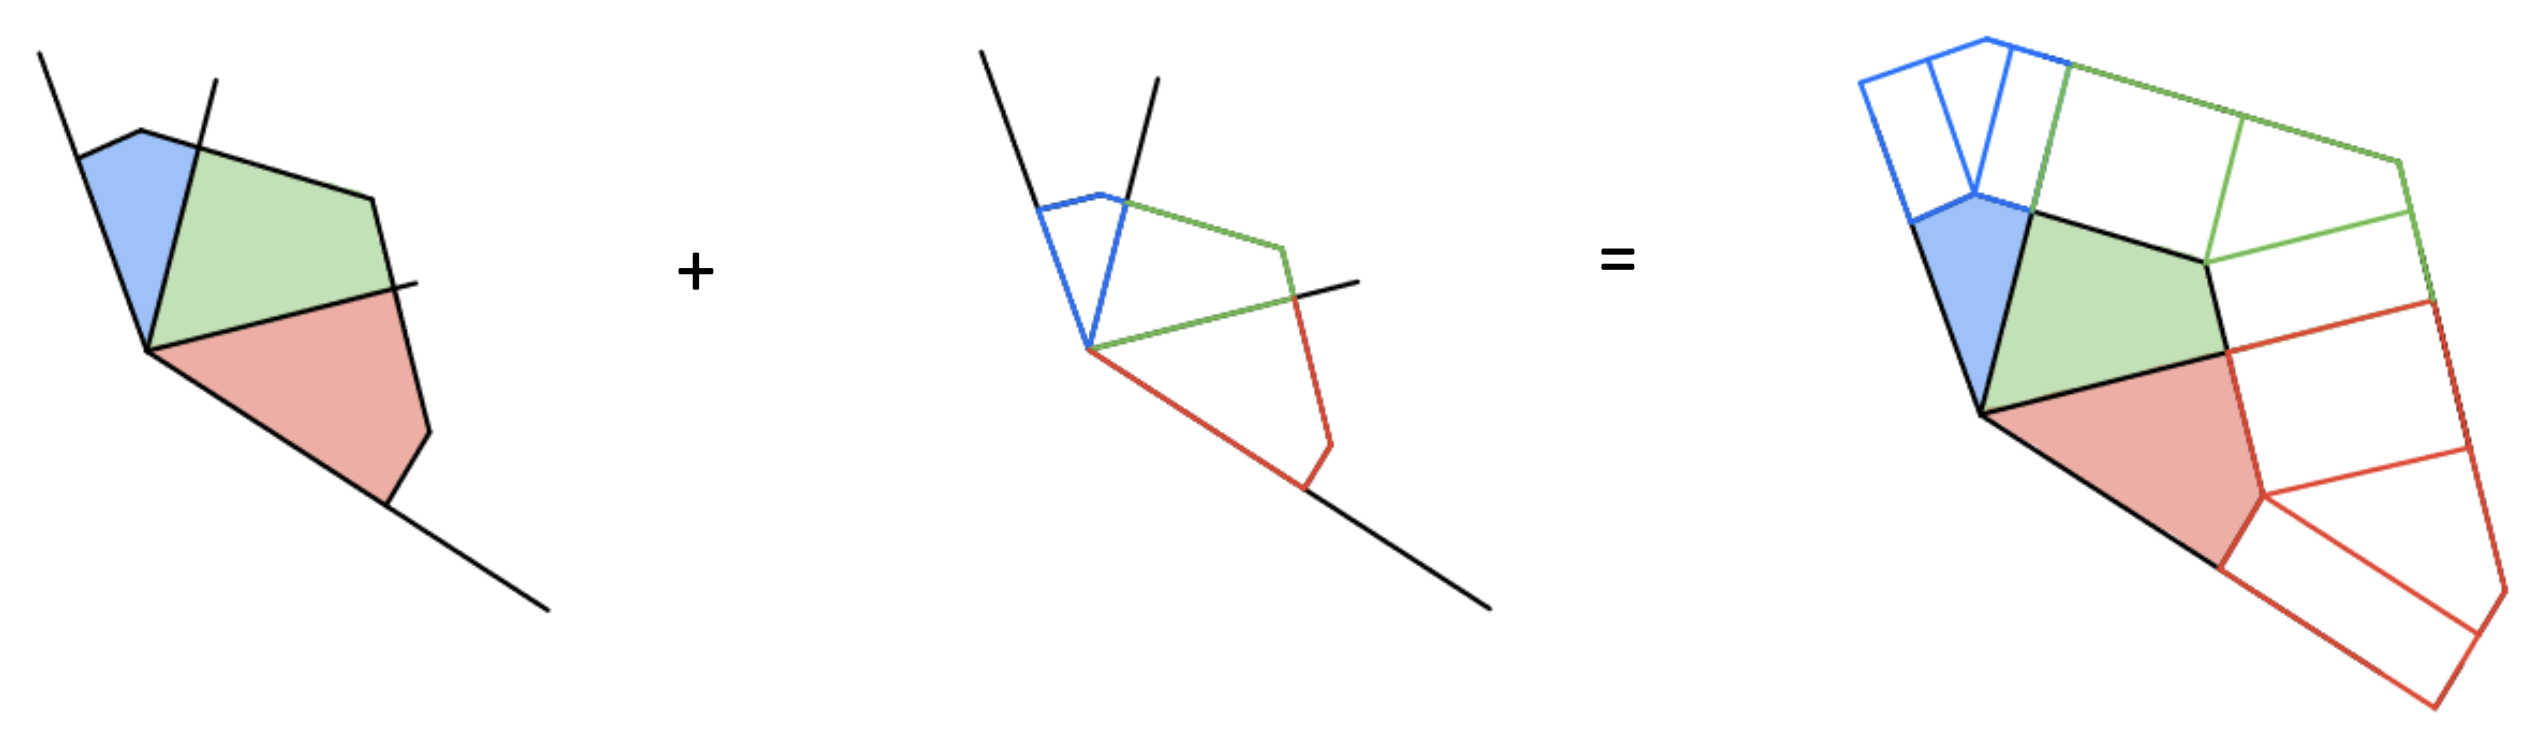
\includegraphics[width=1.05\textwidth]{./images/mvol_ex}
    \caption{Component wise Minkowski sums of two normal complexes of the same fan; note each polytope in the sum is still in its correct cone}
\end{figure}
That this works in general is not obvious.
Nor is it immediate that this newly defined function has all the nice properties of the original mixed volumes.
However, from Proposition~3.1 in \cite{nowakMixedVolumesNormal2023}, we have the following guarantee.
\begin{proposition}
    Let \( \bSigma \subset N \) be a simplicial \( d \)-fan, \( \ast \in \inn(N) \) an inner product on \( \R^n \), and  pseudocubical values \( z_1, \dots, z_n \in \pCub(\bSigma, \ast)\).

    The function
    \[
        \MVol_{\bSigma, \ast}\,:\; \pCub(\bSigma, \ast)^d \to \R_{\geq 0}
    \]
    as defined above has the following properties:
    \begin{enumerate}
        \item \( \MVol_{\bSigma, \ast}(z, z, \dots, z) = \MVol_{\bSigma, \ast}(z) \),
        \item \( \MVol_{\bSigma, \ast} \) is symmetric in all arguments,
        \item \( \MVol_{\bSigma, \ast} \) is multilinear with respect to Minkowski addition in each maximal cone.
    \end{enumerate}

    Further, any function \( \pCub(\bSigma, \ast)^d \to \R_{\geq 0} \)
\end{proposition}
Our new mixed volume function then is well-defined and is uniquely characterized by the same properties as the original.
Theorem~3.6 of \cite{nowakMixedVolumesNormal2023} extends \th\ref{thm:volDegCorrespondence} to a form that lets us evaluate mixed degrees.
\begin{theorem}\th\label{thm:mixedDeg}
    Let \( \bSigma \subset N \) be a balanced \( d \)-fan.
    Choose an inner product \( \ast \in \inn(N) \) and pseudocubical values \( z_1, \dots, z_d \in \pCub( \bSigma, \ast ) \).
    Then
    \[
        \MVol_{\bSigma, \ast}(z_1, \dots, z_d) = \deg\big( D(z_1) \cdots D(z_d) \big).
    \]
\end{theorem}
This is a successful bridge from the realm of geometry back to algebra.
We are now so close to having all the necessary components to prove our main result.
Not only do we have the link between geometry and algebra, it uses the concept of mixed volumes, which are closely related to log-concave sequences.
However, the Alexandrov-Fenchel inequalities are, classically, very dependent on convexity, and normal complexes are decidedly non-convex.

\subsection{Amazing AF Fans}
\todo{should I add a bit more about the recursive structure of normal complexes? It feels not strictly necessary, but then i've gone on lots of not strictly necessary tangents}
Luckily, more recently there have been proofs of the Aleksandrov-Fenchel inequality that make a clearer delineation of the geometric requirements from the rest of the machinery used in the proof.
Using this, \cite{nowakMixedVolumesNormal2023} develops criteria to check which fans will obey inequalities.
\begin{definition}[Alexandrov-Fenchel]\th\label{def:AF}
    Let \( \bSigma \subset N \) be a simplicial \( d \)-fan and \( \ast \in \inn(N) \) an inner product.
    We say that \( (\bSigma, \ast) \) is \emph{Alexandrov-Fencel}, or just \emph{AF}, if \( \Cub(\bSigma, \ast) \neq \emptyset \) and
    \[
        \MVol_{\bSigma, \ast}(z_1, z_2, z_3, \dots, z_d)^2 \geq  \MVol_{\bSigma, \ast}(z_1, z_1, z_3, \dots, z_d)\MVol_{\bSigma, \ast}(z_2, z_2, z_3 \dots, z_d)
    \]
    for all \( z_1, z_2, z_3, \dots, z_d \in \Cub(\bSigma, \ast) \).
\end{definition}
So fans that are AF have exactly the properties we want in generating a log-concave sequence.
The downside, of course, is that having left the convex world, we can't expect every fan to have this property.
If we want to use this in our proof of the main result, we'll need to show that Bergman fans of matroids are AF.
Luckily, we have a theorem from \cite{nowakMixedVolumesNormal2023} that gives us a short list of properties to check.
\begin{theorem}[Nowak-O-Ross 2022]\th\label{thm:suffAF}
    Let \( \bSigma \) be a simplicial  \( d \)-fan, and \( \ast \in \Inn(N_\R) \) an inner product.
    Then \( (\bSigma_\cM, \ast) \) is AF if
    \begin{enumerate}[label=\roman*.]
        \item for every cone \( \sigma \in \bSigma(k) \), with \( k \leq r - 2 \),
              \[
                  \Star(\tau, \bSigma_\cM) \setminus \{ 0 \}
              \]
              is connected,
        \item for each 2-dimensional face of the associated normal complex, \( C(\bSigma, z) \), for some cubical \( z \in \Cub(\bSigma, \ast) \), the quadratic form associated to the volume polynomial has exactly one positive eigenvalue.
    \end{enumerate}
\end{theorem}
We now finally have laid out every piece of the puzzle we'll need to prove our main result.
All that's left is to put them together.

\end{document}

\documentclass[12pt,oneside]{../../sfsuthesis} 
 
\RequirePackage{standalone}
\usepackage[draft]{../../MAThesisOutputFormat}
%====================%
% Packages 
%====================%
%\usepackage{accents}  % Better accents. I'm not using this
\usepackage{enumitem} % Better labels
%\usepackage[explicit]{titlesec}
\usepackage[normalem]{ulem}     % Thing
\usepackage{stackrel} % Stack text nicely
\usepackage{xcolor}   % Nicer Colors

%====================%
% Re-Define 
%====================%
% Sort out the true phi
\def \badphi {\phi}
\def \phi {\varphi}

%====================%
% New Commands 
%====================%
%% Nice Letters
% Blackboard Bold
\newcommand{\R}{\mathbb{R}}
\newcommand{\Z}{\mathbb{Z}}
\newcommand{\bbS}{\mathbb{S}}
% Fancy Math Cal Letters
\newcommand{\I}{\mathcal{I}}
\newcommand{\J}{\mathcal{J}}
\newcommand{\cL}{\mathcal{L}}
\newcommand{\cF}{\mathcal{F}}
% The hipster letters
\newcommand{\sM}{\mathsf{M}}
\newcommand{\bSigma}{\boldsymbol{\Sigma}}
\newcommand{\ow}{\overline{w}}
\newcommand{\oP}{\overline{P}}
\newcommand{\oQ}{\overline{Q}}
\newcommand{\ochi}{\overline{\chi}}
%% Math Operators
\newcommand{\Cub}{\operatorname{Cub}}
\newcommand{\oCub}{\overline{\Cub}}
\newcommand{\Vol}{\operatorname{Vol}}
\newcommand{\oVol}{\overline{\Vol}}
\newcommand{\MVol}{\operatorname{MVol}}
%% Math Symbols
\newcommand{\cl}{\mathrm{cl}}
\newcommand{\rk}{\mathrm{rk}}
\newcommand{\Inn}{\mathrm{Inn}}
\newcommand{\cone}{\mathrm{cone}}

%====================%
% Theorem Environs
%====================%
\newtheorem{dummy}{}[section]
\theoremstyle{definition}
\newtheorem*{Result}{Main Result}

%====================%
% Draft Helpers
%====================%
% \todo : Make a box with todo comments
\newcommand{\todo}[1]{\par \noindent
    \framebox{\begin{minipage}[c]{0.95 \textwidth}
            \textcolor{red}{TO DO:}
            #1 \end{minipage}}\par}
\usepackage[backend=biber,style=numeric]{biblatex}
\addbibresource{../../thesis.bib}

\begin{document}

\chapter{Chapter Title}

\section{Section Name}

\end{document}


%==============%
% Bibliography %
%==============%
\raggedright%
\printbibliography%

\end{document}